%%%%%%%%%%%%%%%%%%%%%%%%%%%%%%%%%%%%%%%%%%%%%%%%%%%%%%%%%%%%%%%%%%%%%%%%%%%%%%%%
%2345678901234567890123456789012345678901234567890123456789012345678901234567890
%        1         2         3         4         5         6         7         8

\documentclass[letterpaper, 10 pt, conference]{ieeeconf}  % Comment this line out if you need a4paper
\usepackage{dsfont,amssymb,amsmath,fancyhdr,mdframed}
\usepackage[dvipsnames]{xcolor}
\usepackage{comment}
\usepackage{dsfont}
\usepackage{graphicx}% 
\usepackage{multicol,lipsum}
%\usepackage{float}
%\usepackage{subfigure}
%\usepackage{geometry}[show frame]
%% Tikz stuff
\usepackage{tikz}
\usepackage{hyperref}
\usepackage{subcaption}
\usetikzlibrary{arrows.meta} % Load arrows.meta for advanced arrow styles
\usetikzlibrary{fit, positioning}
\usetikzlibrary{calc}
\usetikzlibrary{decorations.pathmorphing} 

\tikzstyle{block} = [rectangle, minimum width=1cm, minimum height=1cm, text centered, draw=black]
\tikzstyle{tallblock} = [rectangle, minimum width=.5cm, minimum height=1cm, text centered, draw=black]
\tikzstyle{line} = [thick,-,>=stealth]
\tikzstyle{arrow} = [thick,->,>=stealth]
\tikzstyle{roundedblock} = [rectangle, minimum width=4cm, minimum height=2cm, text centered, draw=black, rounded corners=0.2cm]


\newcommand{\edit}[1]{\textcolor{blue}{#1}}
\newcommand{\emiliosay}[1]{\textcolor{ForestGreen}{[\textsc{Emilio:} #1]}}
\newcommand{\rezasay}[1]{\textcolor{DarkOrchid}{[\textsc{Reza:} #1]}}

\newcommand{\R}{\mathbb{R}}
\newcommand{\N}{\mathbb{N}}
\newcommand{\mc}{\mathcal}
\newcommand{\bs}{\boldsymbol}
\newcommand{\col}{\mathrm{col}}
\newcommand{\buol}{\boldsymbol{u}^{\mathrm{OL}}}
\newcommand{\uol}{u^{\mathrm{OL}}}
\newcommand{\Pol}{P^{\mathrm{OL}}}
\newcommand{\Kol}{K^{\mathrm{OL}}}
\newcommand{\Plqr}{P^{\mathrm{LQR}}}
\newcommand{\Klqr}{K^{\mathrm{LQR}}}
\newcommand{\bu}{\boldsymbol{u}}
\newcommand{\Dx}{D^{\text{x}}}
\newcommand{\Du}{D^{\text{u}}}
\newcommand{\dx}{d^{\text{x}}}
\newcommand{\du}{d^{\text{u}}}
\newcommand{\X}{\mathbb{X}}
\newcommand{\U}{\mathbb{U}}
\newcommand{\red}[1]{\textcolor{red}{#1}}
\newcommand{\VI}{\mathrm{VI}}
\newcommand{\tsum}{\textstyle\sum}
\newcommand{\blkdiag}{\mathrm{blkdg}}
\newcommand{\row}{\mathrm{row}}

\newcommand{\Ms}{M^{\mathrm{s}}}

\newtheorem{theorem}{Theorem}
\newtheorem{definition}{Definition}
\newtheorem{lemma}{Lemma}
\newtheorem{assumption}{Assumption}
\newtheorem{remark}{Remark}
\newtheorem{problem}{Problem}
\newtheorem{corollary}{Corollary}
\newtheorem{fact}{Fact}
\newtheorem{proposition}{Proposition}
%\documentclass[a4paper, 10pt, conference]{ieeeconf}      % Use this line for a4 paper

\IEEEoverridecommandlockouts                              % 

\overrideIEEEmargins                                      % Needed to meet printer requirements.

%In case you encounter the following error:
%Error 1010 The PDF file may be corrupt (unable to open PDF file) OR
%Error 1000 An error occurred while parsing a contents stream. Unable to analyze the PDF file.
%This is a known problem with pdfLaTeX conversion filter. The file cannot be opened with acrobat reader
%Please use one of the alternatives below to circumvent this error by uncommenting one or the other
%\pdfobjcompresslevel=0
%\pdfminorversion=4

% See the \addtolength command later in the file to balance the column lengths
% on the last page of the document

% The following packages can be found on http:\\www.ctan.org
%\usepackage{graphics} % for pdf, bitmapped graphics files
%\usepackage{epsfig} % for postscript graphics files
%\usepackage{mathptmx} % assumes new font selection scheme installed
%\usepackage{times} % assumes new font selection scheme installed
%\usepackage{amsmath} % assumes amsmath package installed
%\usepackage{amssymb}  % assumes amsmath package installed

\title{\LARGE \bf
%Variational Inequalities in Dynamic Games:\\
%Snails, Turtles, or Cheetahs?
A Douglas-Rachford Splitting Method for Solving \\
Monotone Variational Inequalities in Linear-quadratic Dynamic Games
}


\author{Reza Rahimi Baghbadorani, Emilio Benenati, Sergio Grammatico %<-this % stops a space
%\thanks{*This work was not supported by any organization}% <-
\thanks{The authors are with the Delft Center of Systems and
Control (DCSC), TU Delft, the Netherlands. E-mail addresses:
{\tt\small \{r.rahimibaghbadorani, e.benenati,  s.grammatico\}@tudelft.nl}.}%
}


\begin{document}



\maketitle
\thispagestyle{empty}
\pagestyle{empty}


%%%%%%%%%%%%%%%%%%%%%%%%%%%%%%%%%%%%%%%%%%%%%%%%%%%%%%%%%%%%%%%%%%%%%%%%%%%%%%%%
\begin{abstract}
This paper considers constrained linear dynamic games with quadratic objective functions, which can be cast as affine variational inequalities. By leveraging the problem structure, we apply the Douglas-Rachford splitting, which generates a solution algorithm with linear convergence rate. The fast convergence of the method enables receding-horizon control architectures. Furthermore, we demonstrate that \edit{the associated VI admits a closed-form solution within a neighborhood of the attractor, thus allowing for a further reduction in computation time.} Finally, we benchmark the proposed method via numerical experiments in an automated driving application.
\end{abstract}
%%%%%%%%%%%%%%%%%%%%%%%%%%%%%%%%%%%%%%%%%%%%%%%%%%%%%%%%%%%%%%%%%%%%%%%%%%%%%%%%
\section{Introduction}
Dynamic games provide a formal framework for analyzing multi-agent decision-making processes in dynamical systems, where the agents objectives and constraints are coupled through both the system dynamics and their performance criteria \cite{basar_dynamic_1999, haurie2012games}. In such settings, each agent aims to optimize its own cost function while anticipating the actions of other agents, leading to strategic interactions that can be captured via various equilibrium concepts. Dynamic games are an useful model in robust control  \cite{theodor_output-feedback_1996}, as well as robotics \cite{wang_game-theoretic_2021, spica_real-time_2020}, electricity market control \cite{hall_2022} and supply chain strategic organization \cite{hall2024game}. These frameworks enable decentralized decision-making and the analysis of emergent behaviors in complex, multi-agent environments.\\
The desired solution concepts in dynamic games depend on the information structure assumed for the agents. One common approach is the open-loop Nash equilibrium (OL-NE), which defines a trajectory as a sequence of control inputs that is optimal for each agent, given the initial state and the input sequences chosen by the other agents \cite{monti2024feedback,sassano2021constructive}.
{Recent work by \cite{benenati2024linear} demonstrates that the OL-NE of a linear-quadratic dynamic game can be interpreted as the solution to a Linear Quadratic Regulator (LQR) problem formulated in an augmented state space.} In addition, the authors derive a new expression for the achieved agents' objectives and show that the nominal trajectory of a receding-horizon controller with such terminal cost is that of an infinite-horizon OL-NE. Furthermore, the finite-horizon problem used to compute the receding-horizon input is shown equivalent to a linear variational inequality (VI). However, the complexity of the derived VI can increase rapidly as the number of agents, the control horizon and the number of constraints grow, which clashes with the usual requirement of fast online computation. This is where the linear structure of the derived VI should be leveraged to achieve faster convergence, a key contribution of this work. Therefore, let us illustrate the performance of some important state-of-the-art algorithms widely used in solving VI problems, along with a simulation that highlights the contribution of this paper. 
%review some algorithms for solving the VI problem, along with a simulation that highlights the contribution of this paper.
Let us first define the VI problem as follows:
\begin{equation}\label{VI-main}
\text{find} \,\, u^* \in \mathcal{C} \quad \text{s.t.} \, \inf\limits_{u\in \mathcal{C}}\langle F(u^*), u - u^* \rangle \geq 0,
\end{equation}
where $\mathcal{C}\subseteq\R^n$ is a closed, convex set, and $F:\R^n\rightrightarrows \R^n$ is a (in general set-valued) operator. We assume that $F$ is monotone \cite{facchinei2003finite}, Lipschitz, and the solution set of \eqref{VI-main} is nonempty. Note that via the first-order optimality condition, we can rewrite \eqref{VI-main} as a monotone inclusion, $0 \in F(u) + \mathcal{N}_{\mathcal{C}}(u)$, where $\mathcal{N}_{\mathcal{C}}$ is the normal cone of the set \(\mathcal{C}\). This equivalence is beneficial and allows us to use operator splitting methods.\\
%%%%%%%%%%%%%%%%%%%%%%%%%%%%%%%
\begin{comment}
Now, we are in the position to review some recent and closely related existing methods for solving \eqref{VI-main}.\\
%%%%%%%%%%%%%%%%%%%%%%%%%%%%%%%
\textbf{Projected Gradient Descent (PGD) \cite{nemirovskij1983problem}:}  
\begin{align*}
    u^{k+1} &= \pi_{\mathcal{C}}(u^k - \lambda F(u^k)),
\end{align*}
where \(\lambda\) is the stepsize. This method guarantees convergence for strongly monotone operators (with constant \(\mu\)) and Lipschitz operators (with constant \(L\)) when \(\lambda \in (0, 2\mu/L^2)\).\\
\textbf{Extragradient Descent (\red{EXGD}) \cite{malitsky2014extragradient}:}
\begin{align*}
    y^k &= \pi_{\mathcal{C}}(u^k - \lambda F(u^k)), \\
    u^{k+1} &= \pi_{\mathcal{C}}(u^k - \lambda F(y^k)),
\end{align*}
with \(\lambda\) as the stepsize. Unlike PGD, this method ensures convergence for Lipschitz operators (with constant \(L\)) when \(\lambda \in (0, 1/L)\). \\
\textbf{Nesterov's accelerated gradient descent (\red{NAGD}) \cite{nesterov2006solving}:}
\begin{align*}
    u^k &= \arg\max_{u \in \mathcal{C}} \, \sum_{i=0}^k \lambda_i \left[\langle F(y^i), y^i - u \rangle - \frac{\mu}{2} \|u - y^i\|^2\right], \\
    y^{k+1} &= \arg\max_{u \in \mathcal{C}} \, \langle F(u^k), u^k - u \rangle - \frac{\beta}{2} \|u - u^k\|^2,
\end{align*}
where \(\lambda_{k+1} = \frac{\mu}{L} \sum_{i=0}^k \lambda_i\) is the stepsize at iteration \(k+1\). This method guarantees convergence for strongly monotone operators (with constant \(\mu\)) and \(\beta = L\), where \(L\) is the Lipschitz constant of the operator \(F\).\\
\textbf{Projected Reflected Gradient Descent (\red{PRGD}) \cite{malitsky2015projected}:}  
\begin{align*}
    u^{k+1} &= \pi_{\mathcal{C}}(u^k - \lambda F(2u^k - u^{k-1})),
\end{align*}
where \(\lambda\) is the stepsize. This method guarantees convergence for a Lipschitz operator (with constant \(L\)) when \(\lambda \in (0, (\sqrt{2}-1)/L)\). Unlike the extragradient method, it requires only one projection per iteration.\\
\textbf{Golden Ratio Algorithm (GRAAL) \cite{malitsky2020golden}:}  
\begin{align*}
    y^k &= (1-\beta)u^k + \beta y^{k-1}, \\
    u^{k+1} &= \pi_{\mathcal{C}}(y^k - \lambda F(u^k)),
\end{align*}
with \(\lambda\) as the stepsize and \(\beta \in \left(0, (\sqrt{5}-1)/2\right]\). This method ensures convergence for Lipschitz operators (with constant \(L\)) when \(\lambda \in (0, 1/(2\beta L))\) and requires one projection per iteration. Additionally, the stepsize can be chosen adaptively, leading to the Adaptive Golden Ratio Algorithm (aGRAAL) \cite{malitsky2020golden}: 
\begin{align*}
    \lambda_k &= \min\left\{(\beta + \beta^2)\lambda_{k-1}, \frac{\|u^k - u^{k-1}\|^2}{4\beta^2\lambda_{k-2}\|F(u^k) - F(u^{k-1})\|^2}\right\}.
\end{align*}
\textbf{\red{Operator splitting methods (DR)} \cite{facchinei2003finite}:}\\
In these types of methods, the operator \( F \) can be split into a summation of different operators. Then, solving \(\mathrm{VI}(\mathcal{C}, F)\) is equivalent to solving \(0 \in F_1 + F_2\), where \(F + \mathcal{N} = F_1 + F_2\), and the iterative update of each sub-operator leads to convergence towards the solution. A famous class of these algorithms is the Douglas-Rachford splitting method, which can be written as:
\begin{align*}
   y^{k+1} &= (I + \lambda F_2)^{-1}\left(u^k - \lambda F_1(u^k)\right), \\
   u^{k+1} &= u^k + \gamma(y^{k+1} - u^k),
\end{align*}
where $\gamma \in (0,2)$ is a relaxation parameter. The convergence of this method is guaranteed for different cases of $F_1$ and $F_2$; we refer interested readers to~\cite{giselsson2017tight,moursi1805douglas} for further details.
\end{comment}
%%%%%%%%%%%%%%%%%%%%%%%%%%%%%%%%%%%%%
As shown in Section \ref{sec: OL-NE as VI}, {under some technical assumptions, a solution to a constrained linear-quadratic game can be found by solving a strongly monotone affine variational inequality problem} with linear constraints, i.e. $F = Mu + q$ and $\mathcal{C}: Du \leq d$ (where $M$ can be a non-symmetric matrix). Therefore, having efficient methods to solve affine VIs is essential for addressing dynamic game problems (OL-NE). Figure \ref{fig1} presents a comparison of the residuals for six widely used algorithms from the literature: (i) Projected gradient descent (PGD) \cite{nemirovskij1983problem}, (ii) Extragradient descent (EXGD) \cite{malitsky2014extragradient} (iii) Nesterov's accelerated gradient descent (NAGD) \cite{nesterov2006solving} (iv) Projected reflected gradient descent (PRGD) \cite{malitsky2015projected}, (v) adaptive Golden ratio (aGraal) \cite{malitsky2020golden}, and (vi) Operator splitting methods (DR) \cite{facchinei2003finite} (additional details on these algorithms and their update rules available in Appendix \ref{algorithm review}). These algorithms are applied to 10 randomly generated strongly monotone affine VIs, with a non-symmetric matrix $M \in \mathbb{R}^{n \times n}$, a vector $q \in \mathbb{R}^n$, and linear constraints defined by $D \in \mathbb{R}^{m \times n}$ and $d \in \mathbb{R}^{m}$, where $n = 100$ and $m = 20$.\\
\begin{figure}[!h]
     \centering
           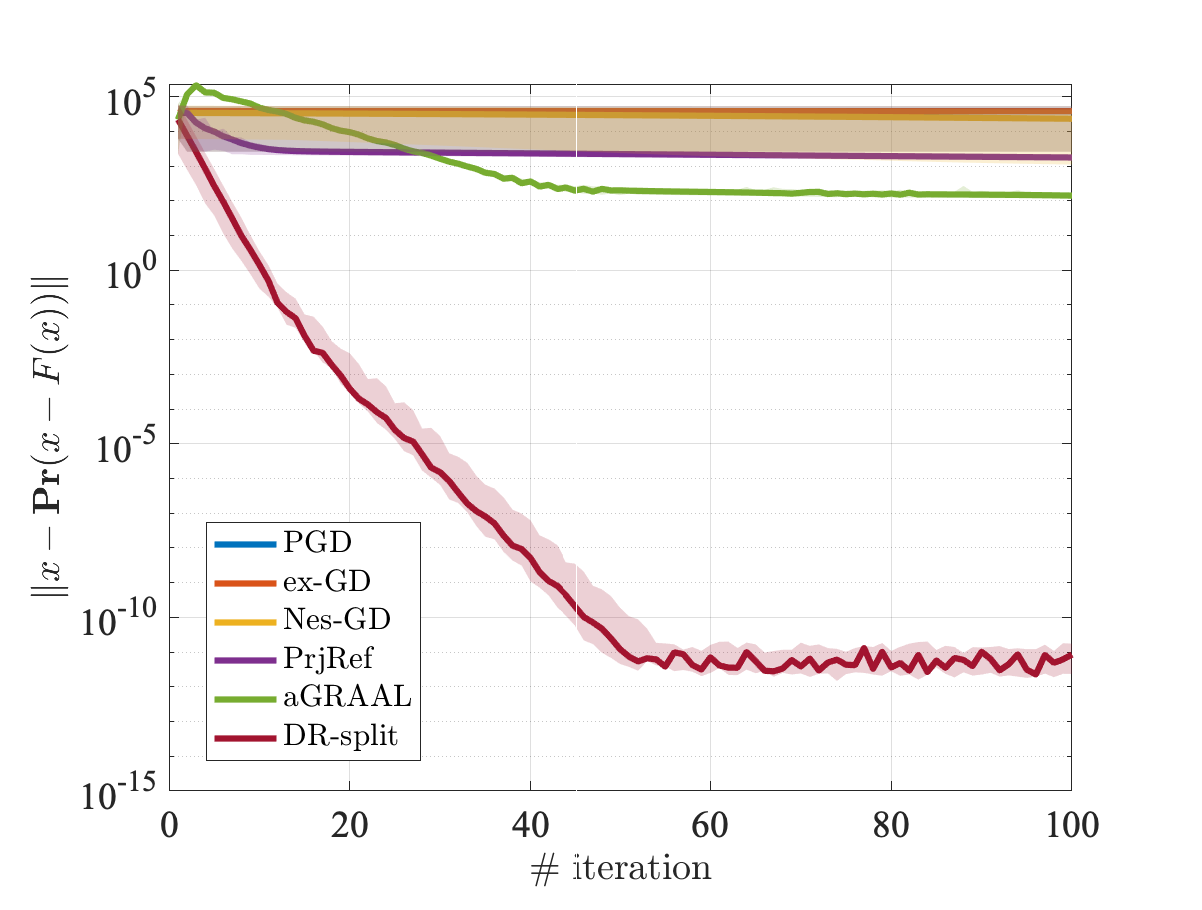
\includegraphics[width=0.45\textwidth]{VImethods.eps}
           \caption{Comparison of residuals for different state-of-the-art VI solution methods.} 
           \label{fig1}
\end{figure}
As illustrated in Figure \ref{fig1}, the splitting method demonstrates superior performance compared to other methods, which motivates leveraging the linear VI structure derived from the dynamical system to achieve faster convergence guarantees. With this in mind, our technical contributions are summarized as follows:
\begin{itemize}
   \item {First, we define a strongly monotone affine VI whose solution, under some technical assumptions, is an infinite open-loop Nash equilibrium for the linear-quadratic dynamic game. We show that the solution to the problem is \edit{known in closed form when the initial state lies in a neighborhood of the origin.}}
   \item Second, we leverage the linearity of the VI in a splitting-type method to improve its solution time. Furthermore, we guarantee linear convergence for the derived affine VI of OL-NE. 
   %and \edit{demonstrate that solving the associated VI requires less effort after a sufficiently large time steps when the constraints are not active.} 
   \item We adopt the aforementioned splitting method in computing the control input of a controller based on the receding-horizon solution to a VI derived by a linear-quadratic dynamic game. The test scenario is that of a set of autonomous vehicles, whose objective is to traverse a crossroad while maintaining a safe distance and speed.
\end{itemize}

\textit{\textbf{Notation.}} 
\paragraph{Matrices} We denote as $I_n$ the identity matrix of size $n$ and as $0_{n,m}$ the zero matrix of size $n\times m$.  The subscripts are omitted when clear from context.  For a set of matrices indexed in $\mc I$, $(M_i)_{i\in\mc I}$, we denote as $\col(M_i)_{i\in\mc I}, \row(M_i)_{i\in\mc I}, \blkdiag(M_i)_{i\in\mc I} $ its column, row and diagonal stack, respectively. We denote $M^{-\top}=(M^{\top})^{-1}$ and the Kronecker product as $\otimes$.
\paragraph{Euclidean spaces and operators} Let $\mathcal{C}$ be the finite-dimensional real vector space with the standard inner product $\langle \cdot, \cdot \rangle$ Euclidean norm.  For $x\in\R^n$ and $Q\succ 0$, we denote $\|x\|_{Q} = \sqrt{x^{\top}Qx}$. The subscript is omitted when $Q=I$. We denote as $\pi_{\mathcal{C}}$ the metric projection onto set $\mathcal{C}$ ($\pi_{\mathcal{C}}(u) = \arg\min_{y \in \mathcal{C}} \|u - y\|$).  We define the normal cone of the set \( \mathcal{C} \) at the point \( u \in  \mathcal{C} \) as $\mathcal{N}_{\mathcal{C}} (u) = \{ g : g^\top u \geq g^\top y, \,\,  \forall y \in \mathcal{C} \}$. An operator $F$ is $L$-Lipschitz, if there is $L>0$ such that for all $u,y \in \mathcal{C}$ we have $\|F(u) - F(y)\| \leq L\|u-y\|$. The operator $F$ is (strongly) monotone if $\langle F(u) - F(y), u - y \rangle \geq  \mu \|u-y\|^2$ for all $u,y \in \mathcal{C}$ and some $\mu \geq 0 (>0)$. For a closed set $\mc C$, we denote its interior as $\mathrm{int}(\mc C)$. {We denote the VI problem \ref{VI-main} with the operator \( F \) and set \( \mathcal{C} \) as \( \mathrm{VI}(\mathcal{C}, F) \).}
\paragraph{Real sequences} We denote as $\mc S^n_T$ a sequence in $\R^n$ with length $T\in\N\cup \infty$. Let $w\in\mc S_T^n$. We denote as $w[t]$, with $t\in\{0,...,T-1\}$, its $t$-th element. If $w: \R^m \to \mc S^n_T$, that is, $w(x)$ is a sequence for all $x\in\R^m$, then we denote as $w[t|x]$ its $t$-th element. We treat finite sequences as column vectors, that is, if $w\in\mc S^n_T$, then $w=\col(w[t])_{t\in\{0,...,T-1\}}$.
\paragraph{Game theory} We consider multi-agent systems, and we denote as $N$ the number of agents. We denote as $\mc I:=\{1,...,N\}$  and as $\mc I_{-i}:=\mc I\setminus\{i\}$. We denote in boldface the column stack over $\mc I$,  e.g. $\bs{w}=\col(w_i)_{i\in\mc I}$. We add the subscript $-i$ to denote the stack over $\mc I_{-i}$, e.g. $\bs{w}=\col(w_i)_{i\in\mc I_{-i}}$. If $w_i\in\mc S_\infty^N$ for all $i\in\mc I$ then, with slight abuse of notation, we denote $\bs{w}:=(w_i)_{i\in\mc I}$, $\bs{w}_{-i}:=(w_i)_{i\in\mc I_{-i}}$. 
%%%%%%%%%%%%%%%%%%%%%%%%%%%%%%%
%\rezasay{I'm not sure if we need this part. We can remove it to save space.}\\
%\textit{\textbf{Roadmap.}} In the rest of the paper, we first establish conditions to formulate the OL-NE as an affine VI problem in Section \ref{sec: OL-NE as VI}. Next, in Section \ref{sec:convergence}, we introduce a Douglas-Rachford splitting-type method to solve the derived VI linearly while ensuring quadratic convergence for each corresponding VI as the time steps increase. Section \ref{sec: simulation} benchmarks our proposed method through several experiments in a \red{vehicle platooning application}. Finally, discussions and future work are provided in Section \ref{sec: conclusion}.
%%%%%%%%%%%%%%%%%%%%%%%%%%%%%%%
\section{Open-Loop Nash Equilibria as Solutions of a Variational Inequality}\label{sec: OL-NE as VI}
We consider a linear system with $N$ inputs, each controlled by a self-interest agent. We denote the sequence of control inputs of agent $i$ as $u_i \in \mc S_{\infty}^m$. The system dynamics is ruled by the difference equation
\begin{equation}\label{eq:dynamics}
    x[t+1] = Ax[t] + \sum_{i\in\mc I} u_i[t].
\end{equation} 
We denote as $\phi(t, x_0, \bu)$ the solution at time $t$ of \eqref{eq:dynamics} with initial state $x_0$ and input $\bu$. We consider quadratic stage costs for all agents:
\begin{equation}
    \ell_i(x[t],u_i[t]):= \tfrac{1}{2}(\|x[t]\|^2_{Q_i} + \|u_i[t]\|^2_{R_i}) \qquad \forall t,
\end{equation}
and linear time-invariant constraints: define the stage-feasible sets as
\begin{align}
    \mathbb{U}_i(\bu_{-i}[t]):=\Large\{ u_i[t]: \sum_{j\in \mc I} \Du_j u_j[t] + \du &\leq 0 \Large\} \\
    \mathbb{X}:= \{x[t]: \Dx x[t]+ \dx \leq 0 \},
\end{align}
and the collective feasible input sequences with length $T\in\N\cup\{\infty\}$ as 
\begin{align*}
        \mc{U}_T(x_0):= \large\{ \bu:~~ &u_i[t] \in \U_i(\bu_{-i}[t]) &\forall i\in\mc I,t<T; \\
         &\phi(t,x_0,\bu) \in\X &\forall t<T\large\}.
\end{align*}
Note that, if $T$ is finite, $\mc U_T(x_0)$ can be expressed as a finite number of linear inequalities by substituting the dynamics to eliminate $\phi$: 
\begin{align}
    \bu&\in\mc U_T(x_0) \iff D\bu + d_{x_0} \leq 0, ~\text{where} \label{def-constraint1}\\ 
    D &:= 
        \row\left(\begin{bmatrix}
            I_T \otimes \Du_i \\
            (I_T\otimes\Dx)\Gamma_i
        \end{bmatrix}\right)_{i\in\mc I} \label{def-constraint2}\\ 
    d_{x_0} &:= \begin{bmatrix}
    \mathds{1}_{T} \otimes d^{\text{u}}\\
    (I_T\otimes \Dx)\Theta x_0 + \mathds{1}_{T} \otimes d^{\text{x}} \end{bmatrix}\label{def-constraint3}\\
    \Theta &:= \col(A^k)_{k\in\{1,...,T\}}, \label{def-constraint4}\\
    \Gamma_i &:= \begin{bmatrix}
            B_i & 0 & \dots & 0 \\
            A B_i & B_i & \dots & 0 \\
            \vdots &  & \ddots & \\
            A^{T-1}B_i & A^{T-2}B_i & \dots  &B_i
        \end{bmatrix}. \label{def-constraint5}
\end{align}
We define the (infinite-horizon) Open-Loop Nash equilibrium (OL-NE) $\buol$ as an input sequence such that the infinite-horizon objective
\begin{equation}
    J_i^\infty(x_0, u_i, \bs{u}_{-i}):= \sum_{t=0}^{\infty} \ell_i\big(\phi(t,x_0,\bu),u_i[t]\big)
\end{equation}
cannot be improved by unilateral modifications by any agent.
\begin{definition}[OL-NE] $\buol\in\mc{U}_{\infty}(x_0)$ is an OL-NE for the initial state $x_0$ if $\lim_{t\xrightarrow{}\infty} \phi(t,x_0,\buol)=0$ and
    \begin{equation}
        J_i^\infty(x_0, \uol_i, \buol_{-i})\leq J_i^\infty(x_0, u_i, \buol_{-i})
    \end{equation}
    for all $u_i$ such that $(u_i, \buol_{-i})\in\mc{U}_\infty(x_0)$.
\end{definition}
In \cite{benenati2024linear}, the authors determine a finite-horizon problem, whose solutions are a truncation of the OL-NE. Furthermore, this problem can be cast as a linear VI. We summarize these results next:
\begin{assumption} \label{as:objective_system} For all $i \in \mc I$, $Q_i=C_i^{\top}C_i \succeq 0$, $R_i = R_i^{\top}\succ 0$; the pairs $(A,B_i)$ and $(A,C_i)$ are stabilizable and detectable, respectively.
\end{assumption}
\begin{assumption}  \label{as:strict_feasibility} The origin is strictly feasible, that is,
    $0\in\mathrm{int}(\X)$; $0\in\mathrm{int}(\U_i(0))$, for all $i \in \mc I$.
\end{assumption}
\begin{assumption} \cite[Assumption 4.9]{monti2024feedback} \label{as:symplectic_matrix}
    $A$ is invertible and the matrix
    \begin{align*}
        H = \begin{bmatrix}
            A + \sum_{j\in\mc I}S_jA^{-\top}Q_j & \mathrm{row}(-S_jA^{-\top})_{j\in\mc I} \\
            \col(-A^{-\top}Q_j)_{j\in\mc I} & I_N \otimes A^{-\top}
        \end{bmatrix},
    \end{align*}
    where $S_i:=B_iR_i^{-1}B_i^{\top}$, has exactly $n$ eigenvalues with modulus strictly less than $1$. An $n$-dimensional invariant subspace of $H$ is complementary to
    \begin{equation*}
        \mathrm{Im}\left( \begin{bmatrix}0_{n\times Nn} \\ I_{Nn} \end{bmatrix} \right).
    \end{equation*}
\end{assumption}
The OL-NE is determined via the following procedure: \\
\emph{1)} Find $(\Pol_i, \Kol_i)_{i\in\mc I}$ that solve the coupled algebraic Riccati equations (ARE) \cite[Eq. 9]{freiling_discrete-time_1999}
\begin{align}
    \Pol_i &= Q_i + A^\top\Pol_i(A +\tsum_{j\in\mc I}B_j \Kol_j) \\
    \Kol_i &= -R_i^{-1}B_i^{\top}\Pol_i(A +\tsum_{j\in\mc I}B_j \Kol_j);
\end{align}
\emph{2)} Find positive semi-definite $(\hat{P}_i)_{i\in\mc I}$ and $(\hat{K}_i)_{i\in\mc I}$ that solve the (uncoupled) AREs \cite[Eq. 15]{benenati2024linear}
\begin{subequations}
    \begin{align}
        \hat{P}_i &= \hat{Q}_i + \hat{A}_i^\top\hat{P}_i(\hat{A}_i+\hat{B}_i \hat{K}_i)\\
        \hat{K}_i &= -R_i^{-1}\hat{B}_i^{\top}\hat{P}_i(\hat{A}_i +\hat{B}_i \hat{K}_i),
    \end{align}
\end{subequations}
where 
\begin{align}
    \begin{split}
        \hat{A}_i &:= \begin{bmatrix}
        A & \tsum_{j\neq i} B_j \Kol_j \\
        0 & A + \tsum_{j\in\mc I} B_j \Kol_j
    \end{bmatrix}, \\
    \hat{Q}_i &:= \blkdiag(Q_i, 0_{n\times n}),\\
    \hat{B}_i &:= \col(B_i, 0_{n\times m}),
    \end{split}
\end{align}
\emph{3)} Solve the finite-horizon equilibrium problem
\begin{align} \label{eq:finite_hor_problem}
\begin{split}
\text{Problem $\mc P_1(x_0)$:}&~ \text{find $\bu^*\in\mc U(x_0)$ such that}\\ 
    \forall i: u_i^* \in \min_{u_i} & ~~J_i(x_0, u_i, \bu^*) \\
    \text{s.t.}&~~ (u_i, \bu^*_{-i})\in\mc U_T(x_0), \\
    J_i(x_u, u_i, \bu^*)&:=\sum_{t=0}^{T-1} \Big\{\ell(\phi(t, x_0, u_i, \bu^*_{-i}), u_i[t]) \Big\}\\ 
    &~~+\frac{1}{2}\left\| \begin{bmatrix}
        \phi(T, x_0, u_i, \bu^*_{-i})\\
        \phi(T, x_0, \bu^*)
    \end{bmatrix} \right\|^2_{\hat{P}_i}\\
\end{split}
\end{align}
for some $T\in\N$. \\
Note that $\hat{P}_i\in\R^{2n\times 2n}$ and $\hat{K}_i\in\R^{m\times 2n}$. Let us introduce the ``terminal set'' $\X_f$ as a forward-invariant, constraint-admissible set for the dynamics 
$$x[t+1]=(A + \tsum_{j\in\mc I} B_j \Kol_j) x[t],$$
that is,
\begin{align} \label{eq:term_set}
\begin{split}
    \X_f:=\{x\in\mathrm{int}(\X): & 
    (A + \tsum_{i\in\mc I} B_i \Kol_i) x\in\X_f; \\
    &\tsum_{i\in \mc I}\Du_i\Kol_i x +\du <0
    \}.
\end{split}  
\end{align}
We underline that this set is not explicitly enforced by a terminal constraint in \eqref{eq:finite_hor_problem}.
\begin{lemma}\cite[Theorem 1]{benenati2024linear}
    Let $\bu^*$ solve $\mc P_1(x_0)$, defined in \eqref{eq:finite_hor_problem}. Let $x_T:=\phi(T, x_0, \bu^*)$ and let $x_T\in \mathbb{X}_f$.
    Then, the sequence defined as
    \begin{equation}
        \forall i: \begin{cases}
            u_i^*[t] & \text{if} ~t < T,\\
            \Kol_i (A + \tsum_j B_j\Kol_j)^{t-T} x_T & \text{if} ~t\geq T
        \end{cases}
    \end{equation}
    is an OL-NE for the initial state $x_0$.
\end{lemma}
Intuitively speaking, if one defines the sequence of inputs
resulting from the linear feedback $(\Kol_j)_{j\in\mc I}$  and the initial state $x_0$
\begin{align}\label{eq:unconstrained_NE_state_sequence}
    u_i^K[t|x_0]&:= \Kol_i (A + \tsum_{j\in\mc I}B_j\Kol_j)^t x_0, & \forall~i, t,
\end{align}
then the sequence $\bu^K(x_0)$ is a OL-NE for the unconstrained system for the initial state $x_0$ \cite[Theorem 4.10]{monti2024feedback}. Furthermore, the function $\frac{1}{2}\left\| \begin{bmatrix}
    x_0\\ y_0
\end{bmatrix} \right\|^2_{\hat{P}_i}$ identifies the $i$-th agent's optimal cost-to-go from state $x_0$, when the remaining agents apply the input sequence $\bu^K_{-i}(y_0)$ \cite[Lemma 1]{benenati2024linear}. 
% This is formalized in the following properties: We remand to \cite[\S 3B]{benenati2024linear} for their derivation.
% \begin{subequations}
%     \begin{align}
%         \left\|\begin{bmatrix}
%             x_0 \\ y_0
%         \end{bmatrix} \right\|_{\hat{P}_i} & \leq J_i^{\infty}(x_0, u_i, \bu^K_{-i}(y_0)) \\
%         \left\|\begin{bmatrix}
%             x_0 \\ x_0
%         \end{bmatrix} \right\|_{\hat{P}_i} &= J_i^{\infty}(x_0, u^K_i(x_0), \bu^K_{-i}(x_0)).
%     \end{align}
% \end{subequations}
Therefore, the terminal cost in \eqref{eq:finite_hor_problem} models the ``tail" of agent's $i$ objective for the terminal states $x[T]$ from which $u_i^K(x[T])$ is feasible, thus allowing one to compute the infinite-horizon constrained OL-NE by solving  a finite-horizon problem. This generalizes a known result in single-agent optimal control \cite{bei_hu_toward_2002}. We now link the solutions to $\mc P_1(x_0)$ and the solutions to a VI. Define the mapping 
\begin{equation} \label{eq:def_F}
        F(\bu, x_0) = M\bu + q,
    \end{equation}
    where
    \begin{align}\label{eq:def_VI_matrices}
    \begin{split}
        M&:= \mathrm{blkdg}(\bar{R}_i)_{i\in\mc I} + \begin{bmatrix}
            \Gamma_1^\top\bar{Q}_1\Gamma_1 & \dots &\Gamma_1^\top\bar{Q}_1\Gamma_N \\
            \Gamma_2^\top\bar{Q}_2\Gamma_1 & \dots & \Gamma_2^\top\bar{Q}_2\Gamma_N \\
            \vdots & \ddots & \\
            \Gamma_N^\top\bar{Q}_N\Gamma_1 & \dots & \Gamma_N^\top\bar{Q}_N\Gamma_N
        \end{bmatrix}, \\
        q&:= \col(\Gamma_i^{\top}\bar{Q}_i\Theta x_0)_{i\in\mc I},\\
        \bar{R}_i&:= I_T\otimes R_i, \qquad \forall i\\
        \bar{Q}_i&:= \blkdiag(I_{T-1}\otimes Q_i, \Pol_i), \qquad \forall i.
    \end{split}
    \end{align}

\begin{align}\label{eq:def_P2}
\begin{split}
    \text{Problem}~ \mc P_2(x_0):~~&\text{find $\bu^*$ that solves}\\&\VI(F(\cdot, x_0), \mc{U}_T(x_0)). 
\end{split}
\end{align}

\begin{lemma}\cite[Proposition 2]{benenati2024linear}\label{lem: OL-NE as VI}
    If $\bu^*$ is a solution to $\mc P_2(x_0)$, then it is also a solution to  $\mc P_1(x_0)$.
\end{lemma}

\begin{figure}
    \centering
    \centering\resizebox{.7\columnwidth}{!}{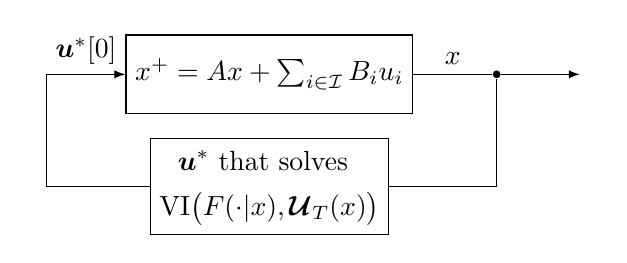
\begin{tikzpicture}[>=latex, node distance=1cm, auto]

    % Nodes
    \node [draw, block] (plant) at (0,0) {$x^+ = Ax + \tsum_{i\in\mc I} B_i u_i$};
    \node [draw, block, below=.3cmof plant] (GNEP) { $\begin{aligned}
        &~~\bu^* \text{ that solves} \\
        &\mathrm{VI}\big(F(\cdot|x), \bs{\mc U}_T(x)\big)
    \end{aligned}$ };

    \node [draw=none, left=of plant] (w) {};
    \node [fill=black, circle, right=of plant, inner sep=1pt] (dot) {};

    \node [draw=none, right=of dot] (x) {};

    % Connections

    \draw[-] (plant.east) --  node[above] {$x$}  (dot.west);
    \draw[-] (dot.south) |- (GNEP.east);
    \draw[->] (dot.east) -- (x.west);
    \draw[-] (GNEP.west) -| (w.east);
    \draw[->] (w.east) -- node[above] {$\bu^*[0]$}  (plant.west);
      
\end{tikzpicture}
}
    \caption{Receding-horizon OL-NE controller}
    \label{fig:block_scheme}
\end{figure}


Lemma \ref{lem: OL-NE as VI} identifies a computational method for the solutions of \eqref{eq:finite_hor_problem}, as efficient algorithms exist for the solution of a VI \cite{facchinei2003finite}. The need for a fast solution algorithm to $\mc P_2$ is of particular relevance, because the authors of \cite{benenati2024linear} propose the receding-horizon control action illustrated in Figure \ref{fig:block_scheme}, based on the recomputation at each timestep of its solution. 
\iffalse
\begin{lemma}
    If for all $i\in\mc I$
    \begin{align} \label{eq:gerschgorin_criterion}
    \begin{split}
    \lambda_{\text{min}}\left(\Gamma_i^{\top}\frac{\bar{Q}_i + \bar{Q}_i^{\top}}{2}\Gamma_i + \bar{R}_i\right) > \sum_{j\neq i} \left\| \Gamma_i^\top\frac{\bar{Q}_i+\bar{Q}_j^{\top}}{2}\Gamma_j \right\|,
    \end{split}
\end{align}
    and $\mc U_T(x_0)$ is non-empty, then $M+M^{\top}\succ 0$ and $VI(F(\cdot, x_0), \mc U_T(x_0))$ admits an unique solution for all $x_0$, where $F,M, (\bar{R}_i,\bar{Q}_i, \Gamma_i)_{i\in\mc I}$ are defined in \eqref{eq:def_F} and \eqref{eq:def_VI_matrices}.
\end{lemma}
\begin{proof}
$F$ admits a unique solution if $M+M^{\top}\succ 0$, following \cite[Proposition 2.3.2]{facchinei_finite-dimensional_2007}. Denote $\Ms = M + M^{\top}$ and consider its block partitioning with block size $Tm\times Tm$. Denote the $i,j$-th element as $\Ms_{i,j}$, with $i,j\in\mc I^2$. Clearly, $\Ms\succ 0$ if and only if $-\Ms$ is Hurwitz. From \cite[Corollary 2.34]{bullo_contraction_2024}, $-\Ms$ is Hurwitz if and only if its Metzler majorant \cite[\S 2.2]{bullo_contraction_2024}, denoted as $\lceil -\Ms \rceil$, is Hurwitz. By definition, 
\begin{equation}
    \lceil -\Ms \rceil = \begin{bmatrix} \mu(-\Ms_{11}) & \|\Ms_{12}\| & ... & \|\Ms_{1N}\| \\
        \|\Ms_{21}\| & \mu(-\Ms_{22}) & ... & \|\Ms_{2N}\| \\
        \vdots &  & \ddots & & \\
        \|\Ms_{N1}\| & \|\Ms_{N2}\| & ... & \mu(-\Ms_{NN}).
    \end{bmatrix}
\end{equation}
where $\mu(\cdot)$ denotes the $\ell_2$ induced log-norm \cite[Eq. 2.23]{bullo_contraction_2024}. Note that $\lceil -\Ms \rceil$ is symmetric, thus it is Hurwitz if and only if $-\lceil -\Ms \rceil\succ 0$. By the Gerschgorin disk theorem \cite[Theorem 2.8]{bullo_lectures_2024}, a sufficient condition is
\begin{equation} \label{eq:gerschgorin}
	-\mu(-\Ms_{ii}) \geq \sum_{j\neq i} \|\Ms_{ij}\| \qquad \forall i.
\end{equation}
From \cite[Example 2.25]{bullo_contraction_2024} and the matrix symmetry, it holds for all $i$ that $\mu(-\Ms_{ii}) = \lambda_{\text{max}}(-\Ms_{ii})$. Since $-\Ms_{ii}$ is negative definite, it holds that $\lambda_{\text{max}}(-\Ms_{ii}) = -\lambda_{\text{min}}(\Ms_{ii}) $. The statement immediately follows from \eqref{eq:gerschgorin}.
\end{proof}
In particular, \eqref{eq:gerschgorin_criterion} holds if $R_i=r_iI_m$, with $r_i>0$ large enough for all $i$. The resulting closed-loop system 
\begin{equation}\label{eq:closed_loop_dyn}
    x[t+1] = Ax[t] + \sum_{j\in\mc I} B_j \kappa_j(x[t]).
\end{equation}
is asymptotically stable, and its nominal dynamics is an infinite-horizon OL-NE following Lemma \ref{le:inf_hor_OLNE} and \cite[Lemma 2]{benenati2024linear}. 
\fi
 %In Section \ref{sec:convergence}, we show \edit{its quadratic convergence} when  
 \edit{Following the asymptotic stability of the closed-loop system \cite[Theorem 2]{benenati2024linear} and Assumption \ref{as:strict_feasibility}, the state will belong to a neighborhood of the origin where the constraints are inactive, after a sufficiently long time evolution: This is relevant as it allows one to derive a closed-form solution for the solution of $\mc P_2(x_0)$ in a neighborhood of the origin, thus reducing the computational complexity needed for implementing the controller in Figure \ref{fig:block_scheme}.}
\begin{lemma}\label{lem: inactive cons}
    Let $x_0\in \mathbb{X}_f$. Let $M+M^{\top}\succ 0$. Let $\bu^*$ solve $\mc P_2(x_0)$. Then, the unique solution to $\mc P_2(x_0)$ is  $\bar{\bu}^K$ defined as
    \begin{equation}
    \label{eq:def_bar_u_K}
    \bar{\bu}^K:=(\bu^K[0|x_0], ..., \bu^K[T-1|x_0]).
    \end{equation} 
\end{lemma}
\begin{proof}
    Note that, from the definition of $\X_f$, $\bar{\bu}^K$ is strictly feasible, that is, $\bar{\bu}^K\in\mathrm{int}(\mc U_T(x_0))$. We show that $\bar{\bu}^K$ solves $\mc P_1(x_0)$. Consider a generic sequence $v_i\in\mc S_T^m$. Proceeding by contradiction, we assume
    \begin{equation}\label{eq:contradiction_assumption}
        J_i(x_0, v_i, \bar{\bu}^K) < J_i(x_0,\bar{u}_i^K,\bar{\bu}^K).
    \end{equation}
    Denote $x^v_T = \phi(T, x_0, v_i, \bar{\bu}_{-i}^K)$ and $x^K_T = \phi(T, x_0, \bar{u}_i^K, \bar{\bu}_{-i}^K)$. 
    Following \cite[Lemma 1]{benenati2024linear}, the infinite sequence $w_i$ defined as
    \begin{equation}
        w_i[t]  = \hat{K}_i \left(\hat{A}_i + \begin{bmatrix}
            B_i \\0
        \end{bmatrix} \hat{K}_i\right)^t \begin{bmatrix}
            x_T^v \\ x_T^K
        \end{bmatrix} \quad \forall t\in\N
    \end{equation}
    achieves for agent $i$ the infinite-horizon objective $\tfrac{1}{2}\left\|\begin{bmatrix} 
            x_T^v \\ x_T^K
        \end{bmatrix} \right\|^2_{\hat{P}_i}$ when the other agents apply the sequence $\bu^K_{-i}(x_T^K)$ defined in \eqref{eq:unconstrained_NE_state_sequence}, that is,
    \begin{equation}
        \frac{1}{2}\left\|\begin{bmatrix}
            x_T^v \\ x_T^K
        \end{bmatrix} \right\|^2_{\hat{P}_i} = \sum_{t=0}^\infty \ell(\phi(t, x_T^v, w_i, \bu^K_{-i}(x_T^K)) , w_i[t] ).
    \end{equation}
    Denote as $v_i^{\infty}$ the concatenation of $v_i$ and $w_i$. 
    Substituting the latter in the definition of $J_i$ in \eqref{eq:finite_hor_problem},
    \begin{align} 
    \begin{split}
        J_i(x_0, v_i, \bar{\bu}^K) =& \tsum_{t=0}^{T-1} \ell(\phi(t, x_0, v_i, \bar{\bu}^K_{-i}), v_i[t] ) \\
        +&\tsum_{\tau=0}^{\infty} \ell(\phi(\tau, x_T^v, w_i, \bu^K_{-i}(x_T^K)) , w_i[\tau] ) \\
        =& J_i^\infty(x_0,v_i^\infty, \bu^K_{-i}(x_0)),
    \end{split}
    \end{align}
    where in the latter equality we noted that $\bu^K(x_0)$ is the concatenation of $\bar{\bu}^K$ and $\bu^K(x^K_T)$. Similarly, one can show
    \begin{equation}
        J_i(x_0, \bar{u}_i^K, \bar{\bu}^K) = J_i^\infty(x_0, u^K_i(x_0), \bu_{-i}^K(x_0)).
    \end{equation}
    Thus, \eqref{eq:contradiction_assumption} implies 
    $$J_i^\infty(x_0,v_i^\infty, \bu^K_{-i}(x_0)) < J_i^\infty(x_0, u^K_{i}(x_0), \bu^K_{-i}(x_0)),$$
    which contradicts the fact that $\bu^K(x_0)$ is an unconstrained OL-NE \cite[Prop. 1]{benenati2024linear}. We conclude that $\bar{\bu}^K$ solves $\mc P_1(x_0)$. Because $\bar{\bu}^K$ is a strictly feasible solution, the optimality conditions applied to $\mc P_1(x_0)$ lead to
    \begin{equation}\label{eq:gradient_is_zero}
        \nabla_2 J_i(x_0, \bar{u}_i^K, \bar{\bu}^K)  = 0, \quad \forall ~i
    \end{equation}
    where, in the latter, $\nabla_{2}$ denotes the partial gradient with respect to the second argument. By algebraic steps \cite[Proof of Prop. 2]{benenati2024linear}, we have
    \begin{equation}
        F(\bar{\bu}^K, x_0) = \col(\nabla_{2} J_i(x_0, \bar{u}_i^K, \bar{\bu}^K))_{i\in\mc I}.
    \end{equation}
     By combining \eqref{eq:gradient_is_zero} and the definition of $\mc P_2(x_0)$ in \eqref{eq:def_P2}, we conclude that $\bar{\bu}^K$ solves $\mc P_2(x_0)$. The statement follows by the uniqueness of the solution to $\mc P_2(x_0)$ \cite[Prop. 2.3.2, Th. 2.3.3]{facchinei2003finite}.
    \end{proof}
    With the receding-horizon control application in Figure \ref{fig:block_scheme}, in the remainder of this paper we explore a Douglas-Rachford (DR) splitting algorithm, which exploits the linear structure of the VI for its fast solution. This algorithm is linearly convergent \cite[Proposition 6]{ferris1996operator} when $M+M^{\top}\succ 0$, and it is advantageous compared to other commonly used VI solution methods, as illustrated in Figure \ref{fig1}.

%%%%%%%%%%%%%%%%%%%%%%%%%%%%%%%%%%%%%%%%%%%%%%%%%%%%%%%%%%%%%%%%%%%%%%%%%%%%%%%%
\section{Algorithm and Convergence}\label{sec:convergence}
\edit{
Consider the following Douglas-Rachford splitting method
\begin{subequations}\label{DR-affineVI} applied to the VI that defines problem $\mc P_2(x_0)$, with $x_0\in\X$:
\begin{align}
    y^{k} &= \arg\min_{y\in\mc U_T(x_0)} \tfrac{1}{2}\|y\|_{(H+M_1)}^2 + \langle q+(M_2 - H)u^k, y \rangle, \label{DR-affineVI-1}\\
    u^{k+1} &= (H+M_2)^{-1}\left(H(2\lambda_k y^{k} + (1-2\lambda_k)u^k) + M_2u^k\right), \label{DR-affineVI-2}
\end{align}
\end{subequations}
where $M_1, M_2, H$ are generic matrices such that:
\begin{align}\label{eq:conditions_convergence}
    \begin{split}
        M_1 = M_1^{\top} &\succeq 0, \, M_2 \succ 0,\\
        M_1 + M_2 &= M,\\
        H = H^{\top} &\succ 0,
    \end{split}
\end{align}
with $M, q$ defined in \eqref{eq:def_VI_matrices}. Note that the $\arg\min$ operation in \eqref{DR-affineVI-1} is single-valued following the fact that $M_1+H$ is positive definite. A suitable choice for $M_1$, $M_2$ when $M\succ 0$ is, for example:
\begin{align}\label{eq:example_matrix_splitting}
    \begin{split}
        M_1^{\text{ex}} &= (M + M^{\top}) / 4, \\ 
        M_2^{\text{ex}} &= (M + M^{\top}) / 4 + (M - M^{\top}) / 2.
    \end{split}
\end{align} In this section, we first establish the linear convergence of the iteration in \eqref{DR-affineVI} to the solution of $\mc P_2(x_0)$ when matrices $M_1$ and $M_2$ are chosen according to \eqref{eq:conditions_convergence}. } 
%%%%%%%%%%%%%%%%%%%%%%%%%%%%%%
\begin{lemma}[{Linear convergence \cite[Proposition 6]{ferris1996operator}}]\label{li-conv}
    {\edit{The sequence $(u_k)_{k\in\N}$ generated by the iteration in \eqref{DR-affineVI} converges linearly \cite[Eq. 5.8]{bauschke_convex_2017} to the unique solution of \(\mathrm{VI}(\mc U_T(x_0), F(\cdot, x_0))\) if $M_1, M_2, H$ satisfy \eqref{eq:conditions_convergence} and $\lambda_k \in (0,1]$ for all $k$.}}
\end{lemma}
\begin{proof}
{\edit{One can show that \eqref{DR-affineVI} is equivalent to the iteration in \cite[Eqq. 30,31]{ferris1996operator}, following the equivalence of a QP to a VI \cite[\S 1.3.1]{facchinei2003finite}. The result then follows directly from case 2 in \cite[Proposition 6]{ferris1996operator}.}}    
\end{proof}
%%%%%%%%%%%%%%%%%%%%%%%%%%%%%%%%%%%%%%
{\edit{At every iteration, the splitting in \eqref{DR-affineVI} requires the solution to a QP, which can be computed efficiently. }
\begin{comment}
\emiliosay{This following discussion feels redundant to me, and not very clear. What is the message that you want to convey?}\rezasay{actually if we remove this part, the theoretical part becomes a bit short, I just want to more emphasize on choosing $M_1$ and $M_2$ in our application} Fortunately, the dynamics of the OL-NE and the corresponding VI in Lemma \ref{lem: OL-NE as VI} provide us with the opportunity to properly choose the symmetric positive semidefinite matrix \( M_1 \) and the positive definite matrix \( M_2 \) (which is not necessarily symmetric) to achieve a fast linear convergence rate, e.g., the choice of $M_1$ and $M_2$ in \eqref{eq:example_matrix_splitting}. Therefore, based on Lemma \ref{li-conv}, we can conclude the linear convergence to the set of solutions of the affine VI derived in the OL-NE problem.
\end{comment}
%, which satisfy the proposed properties.
%%%%%%%%%%%%%%%%%%%%%%%%%%%%%%%%%%%%%
\begin{comment}
\begin{align*}
    M_1 = \mathrm{blkdg}(\bar{R}_i)_{i\in\mc I}, \,\, M_2 = \begin{bmatrix}
            \Gamma_1^\top\bar{Q}_1\Gamma_1 & \dots &\Gamma_1^\top\bar{Q}_1\Gamma_N \\
            \Gamma_2^\top\bar{Q}_2\Gamma_1 & \dots & \Gamma_2^\top\bar{Q}_2\Gamma_N \\
            \vdots & \ddots & \\
            \Gamma_N^\top\bar{Q}_N\Gamma_1 & \dots & \Gamma_N^\top\bar{Q}_N\Gamma_N 
        \end{bmatrix},
\end{align*}
where $\bar{R}_i$, $\bar{Q}_i$, and $\Gamma_i$ are defined in \eqref{eq:def_VI_matrices}. 
%The following lemma provides the linear convergence of the iterative method \eqref{DR-affineVI} for the affine VI, where $M$ can be written as $M = M_1 + M_2$.
\end{comment}
%%%%%%%%%%%%%%%%%%%%%%%%%%%%%%
\begin{comment}
\emiliosay{The new choice of the splitting has nothing to do with the structure of the OL-NE problem. Can we just eliminate Proposition 1? It is basically Lemma 4}
\begin{proposition}[Convergence of derived VI from OL-NE]\label{prop: li-conv-VI in OL_NE}
   {\edit{The iterations in the iterative method \eqref{DR-affineVI} for the affine \( \mathrm{VI}(\mathcal{C}, F) \), derived from the OL-NE problem, converge to the solution linearly.}}
\end{proposition}
\begin{proof}
   {By using the equivalent solution of OL-NE as an affine VI with operator \(F(u) =  Mu + q \) and the constraint set $\mathcal{C}: Du + d_{x_0} \leq 0$, where $M$ and $q$ are defined in \eqref{eq:def_VI_matrices} and the set $\mathcal{C}$ is defined in \eqref{def-constraint1}-\eqref{def-constraint5} (as stated in Lemma \ref{lem: OL-NE as VI}), we can split \( M = M_1 + M_2 \) as follows:
   \begin{align*}
       M_1 = \frac{(M + M^\top)}{4}, \quad M_2 = \frac{(M - M^\top)}{2} + \frac{(M + M^\top)}{4}.
   \end{align*}
    Note that for matrix $M$ in\eqref{eq:def_VI_matrices} we have
    \begin{align*}
        x^\top (M - M^\top)x = 0, \,\, \forall x,
    \end{align*}
    thus $(M - M^\top)\succeq 0$ and $(M + M^\top)\succ0$. Now, it is sufficient to use Lemma \ref{li-conv}, which establishes linear convergence.}
\end{proof}
\end{comment}
%%%%%%%%%%%%%%%%%%%%%%%%%%%%%%%%%%%%%%
\begin{comment}
%\begin{proof}
  We use Theorem 6.5 from \cite{giselsson2017tight}, where the author proves the linear convergence rate of the Douglas-Rachford-type method \eqref{DR-affineVI} for finding the zero of the sum of two maximally monotone operators, i.e., $0 \ni T_1(x) + T_2(x)$, where $T_1(x)$ is a strongly monotone operator. \\
  By noting that solving the VI with operator $F$ on the set $\mathcal{C}$ is equivalent to solving $0 \ni F(x) + \mathcal{N}_\mathcal{C}(x)$, we deduce that the solution to \eqref{} satisfies $0 \ni M_1(x) + M_2(x) + q + \mathcal{N}_\mathcal{C}(x)$. Given the positive definiteness of $M_1$ and the maximal monotonicity of $M_2(x) + q + \mathcal{N}_\mathcal{C}(x)$, as stated in Proposition 1 of \cite{ferris1996operator}, and the linear convergence result from Theorem 6.5 in \cite{giselsson2017tight}, we can conclude the linear convergence of the residual VI \eqref{}.
%\end{proof}
\end{comment}
%%%%%%%%%%%%%%%%%%%%%%%%%%%%%%%%%%%%%%

% We are now in a position to show quadratic convergence of the corresponding VI in OL-NE when the constraints are not active.
% \begin{theorem}[Local quadratic convergence]\label{th: quad-conv} \edit{The sequence $(u_k)_{k\in\N}$ generated by the iteration in \eqref{DR-affineVI} converges quadratically to the unique solution $\bu^*$ of \(\mathrm{VI}(\mc U_T(x_0), F(\cdot, x_0))\) associated with problem $\mc P_2(x_0)$, that is,
%    \begin{equation}
%     \lim\limits_{k \to \infty} \frac{\|u_{k+1} - u^*\|}{\|u_{k} - u^*\|^2} = c, \, c \in (0,1),
%    \end{equation}
%    when $\bu^*\in\mathrm{int}(\mc U_T(x_0))$.}
% \end{theorem}
% \begin{proof}
%    %The proof is straightforward. By applying Lemma \eqref{} we know that the solution is in the interior of the feasible set. Then, the problem reduces to solving a linear system of equations, $Mx + q \ni 0$. Now, by selecting a sufficiently small $H$ in the iterative method \eqref{DR-affineVI}, it becomes like Newton method for solving a linear system of equations which has at most quadratic complexity for strongly monotone VI \cite{taji1993globally,marcotte1987note}.
%    By applying Lemma \ref{lem: inactive cons}, we know that the solution of affine \(\mathrm{VI}(\mathcal{C}, F)\) lies in the interior of the feasible set $\mathcal{U}(x_0)$ \edit{when $x_0\in\X_f$.} Then, it is not difficult to see that the problem reduces to solving a linear system of equations, $0 \in Mu + q$. Now, by selecting a sufficiently small $H$ in the iterative method \eqref{DR-affineVI}, it becomes similar to the Newton method for solving a linear system of equations, which has a quadratic convergence  \cite[Chapter 2]{greenbaum1997iterative}.
% \end{proof}
% We also refer interested readers to \cite{taji1993globally,marcotte1987note} where the authors use the Newton method to solve monotone VIs and show quadratic convergence for strongly monotone VIs in different scenarios.
%%%%%%%%%%%%%%%%%%%%%%%%%%%%%%%%%%%%%%%%%%%%%%%%%%%%%%%%%%%%%%%%%%%%%%%%%%%%%%%%
\section{Numerical Experiments}\label{sec: simulation}
We test the Douglas-Rachford algorithm {with $H=I$, $\lambda_k = 0.5~ \forall k$, \edit{and $M_1$, $M_2$ chosen as in \eqref{eq:example_matrix_splitting}} } on the receding-horizon control architecture in Figure \ref{fig:block_scheme}, applied to the control of autonomous vehicles driving through a crossroad. The vehicles traverse the intersection in the sequence of their arrival. Each vehicle aims to maintain a safe distance from the preceding vehicle intersecting their path, while matching its velocity. If no preceding vehicle intersects their path,  the agent is called a \emph{leading vehicle}, and its objective is to maintain a reference speed. We denote the set of leading vehicles as $\mc{L}$ and the preceding vehicle intersecting the path of $i$ as $\chi(i)$. {We simulate $N=15$ vehicles, with directions
\begin{align*}
    \{&\mathrm{NS}, \mathrm{ES}, \mathrm{WE}, 
    \mathrm{NW}, \mathrm{WN}, \mathrm{WN},
    \mathrm{WS}, \mathrm{NE}, \\
    &\mathrm{NE},
    \mathrm{EW}, \mathrm{NS}, \mathrm{ES}, \mathrm{WS}, \mathrm{SW}, \mathrm{WE}\}
\end{align*}
where \textrm{NS} denotes ``from North to South'' and so on.} For example: Agent 1 is a leading agent; Agent 2 must maintain a safe distance from Agent 1 because the paths \textrm{NS} and \textrm{ES} intersect, thus $\chi(2)=1$; Agent 4 (\textrm{NW}) must maintain a safe distance from Agent 1 (\textrm{NS}), because the path of agent 4 does not intersect with the ones of agents 2,3, thus $\chi(4)=1$. \\
We define $x=\col(x_i)_{i\in\mc I}$, where the state of each vehicle $x_i$ is
\begin{equation}
    x_i = \begin{cases} v^{\text{ref}} - v_i & \text{if}~i\in\mc L\\
        \begin{bmatrix}
            p_{\chi(i)} - p_i - d_i \\
            v_{\chi(i)} - v_i
    \end{bmatrix}  & \text{if}~i\notin\mc L.
    \end{cases}
\end{equation}
%%%%%%%%%%%%%%%%%%%%%%%%%
\begin{figure*}
    \centering
    \captionsetup{justification=centering}
    \subfloat[Agents 1--4 approach the intersection.]{\label{sub-fig1}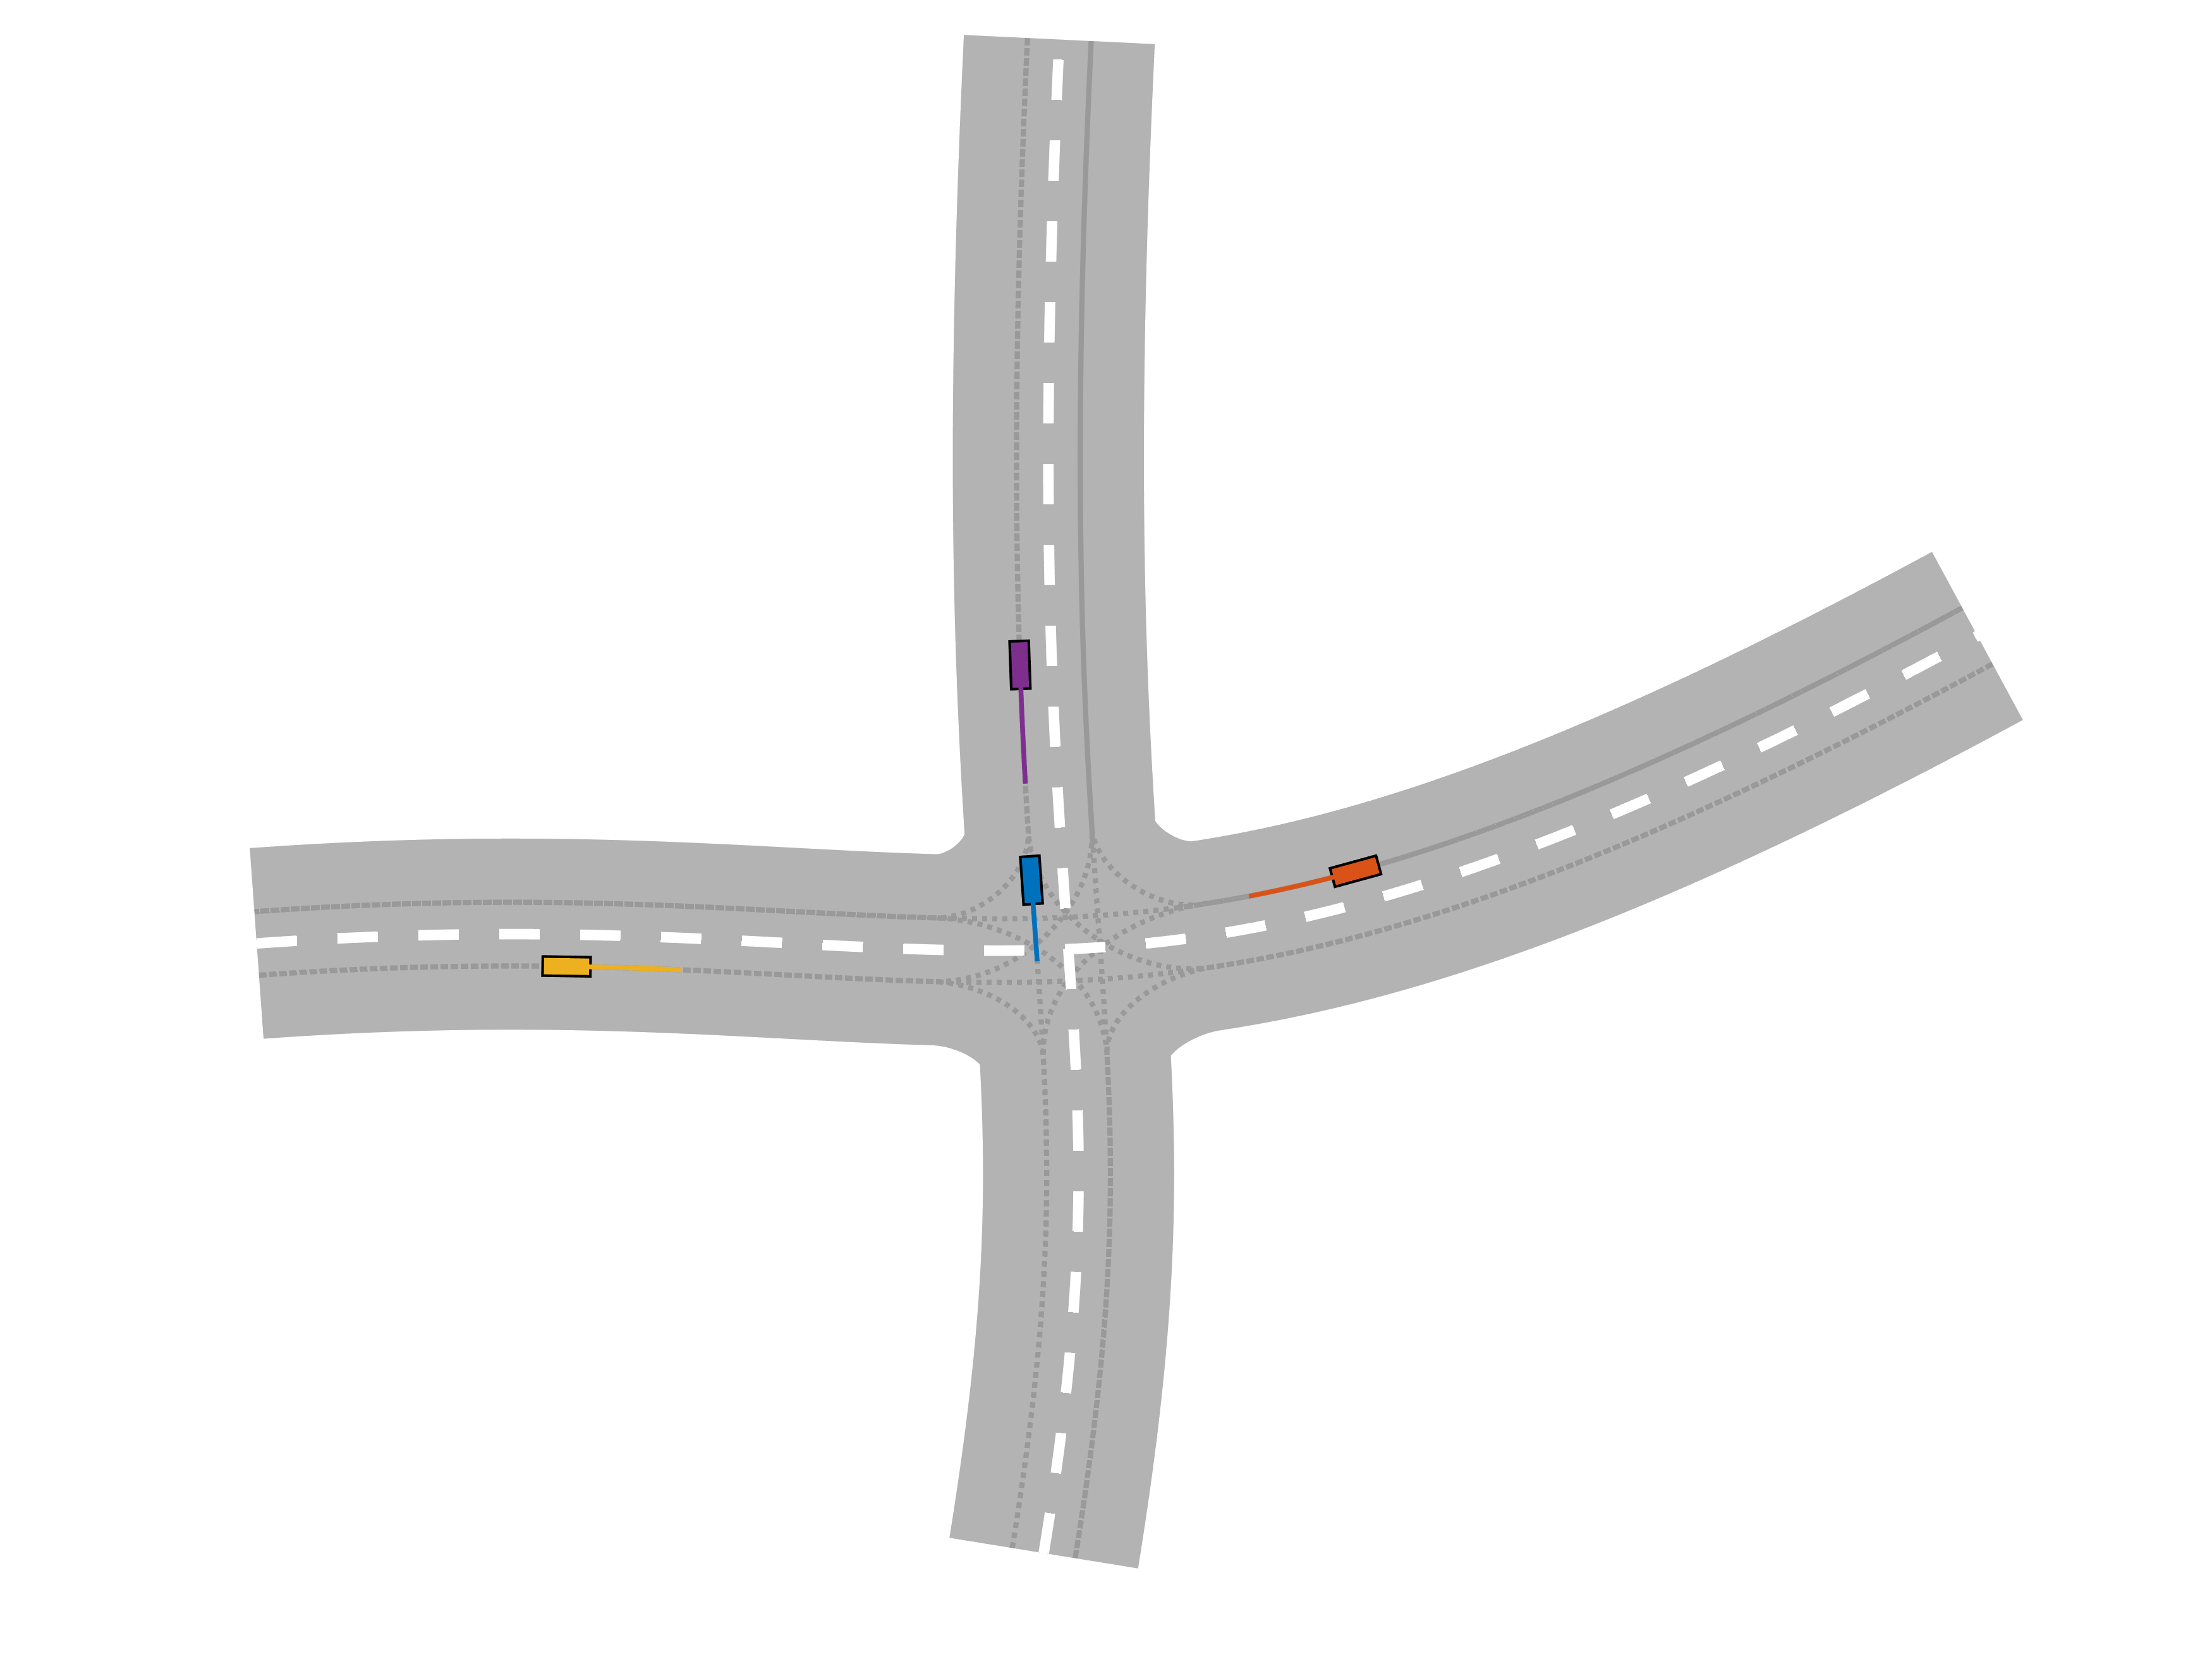
\includegraphics[scale=0.36]{Simulations/frame_crossroad_3.png}}
    \hspace{3mm}
    \subfloat[Agent 1 (Blue) crosses the intersection first. Agents 2 (orange), and 4 (violet) cross next, contemporarily.]{\label{sub-fig2}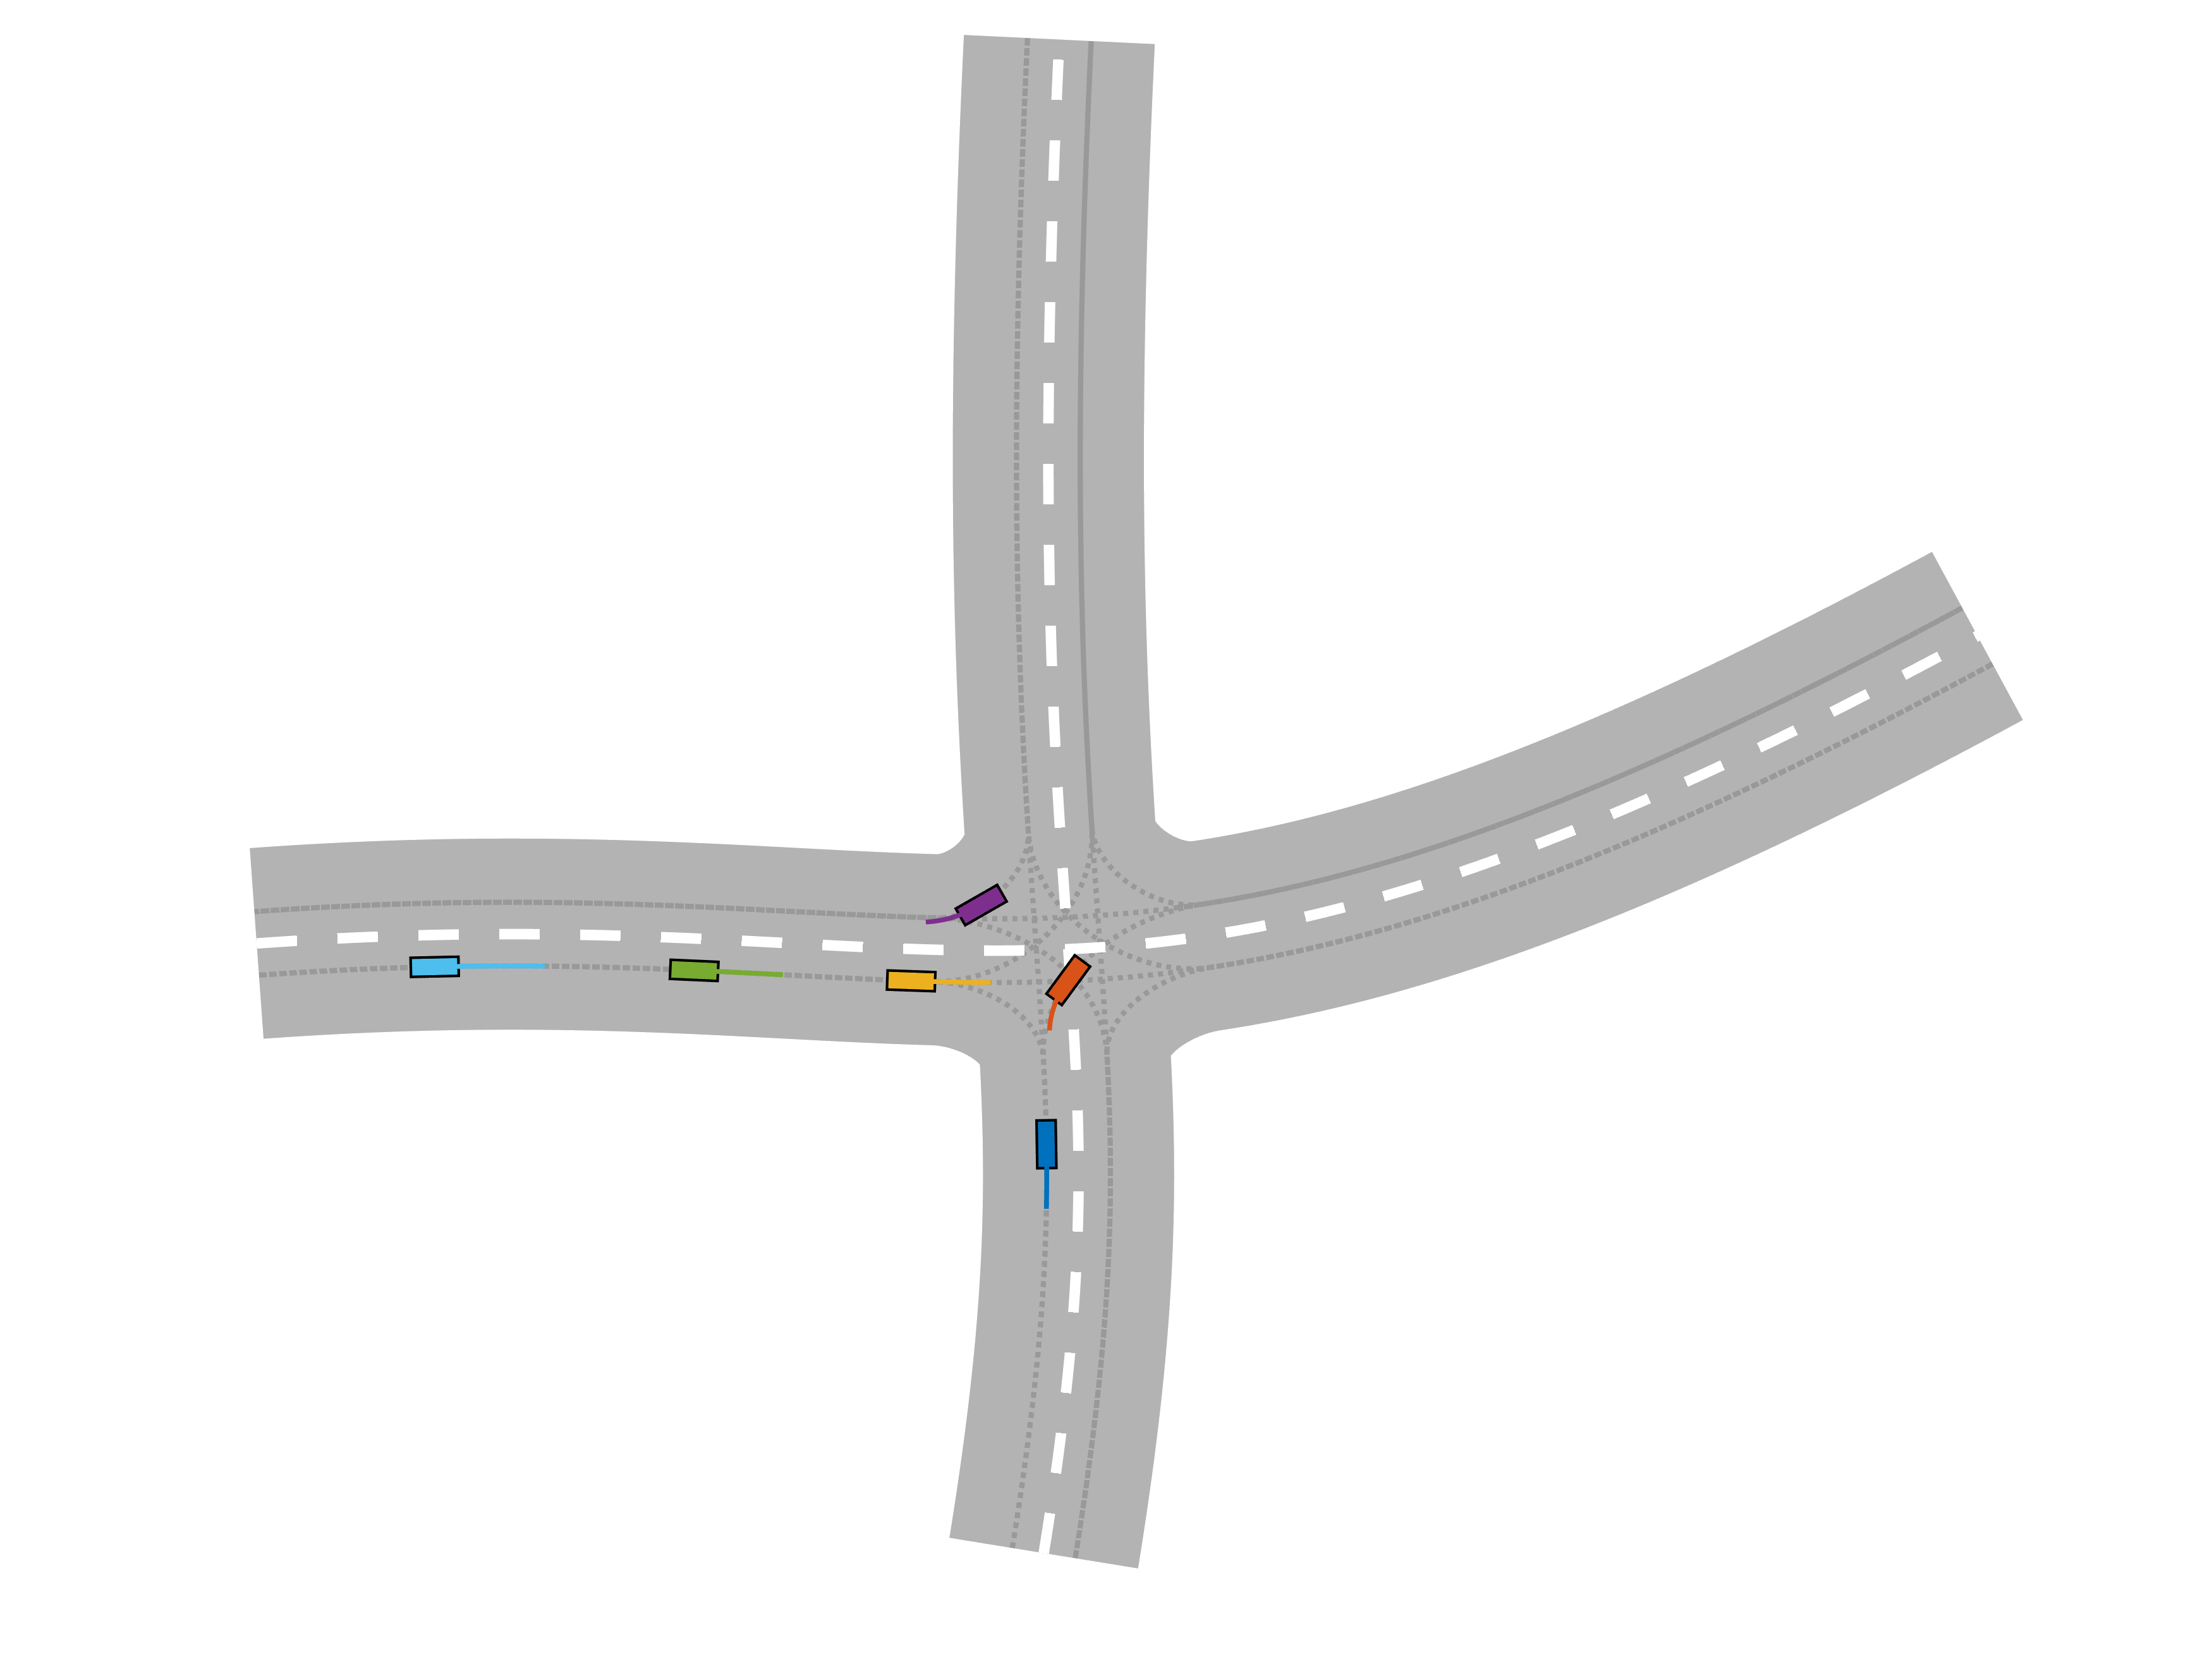
\includegraphics[scale=0.36]{Simulations/frame_crossroad_5.png}
    \hspace{3mm}}
    \subfloat[Agent 3 (yellow) crosses the intersection, followed by Agent 5 (green).]{\label{sub-fig3}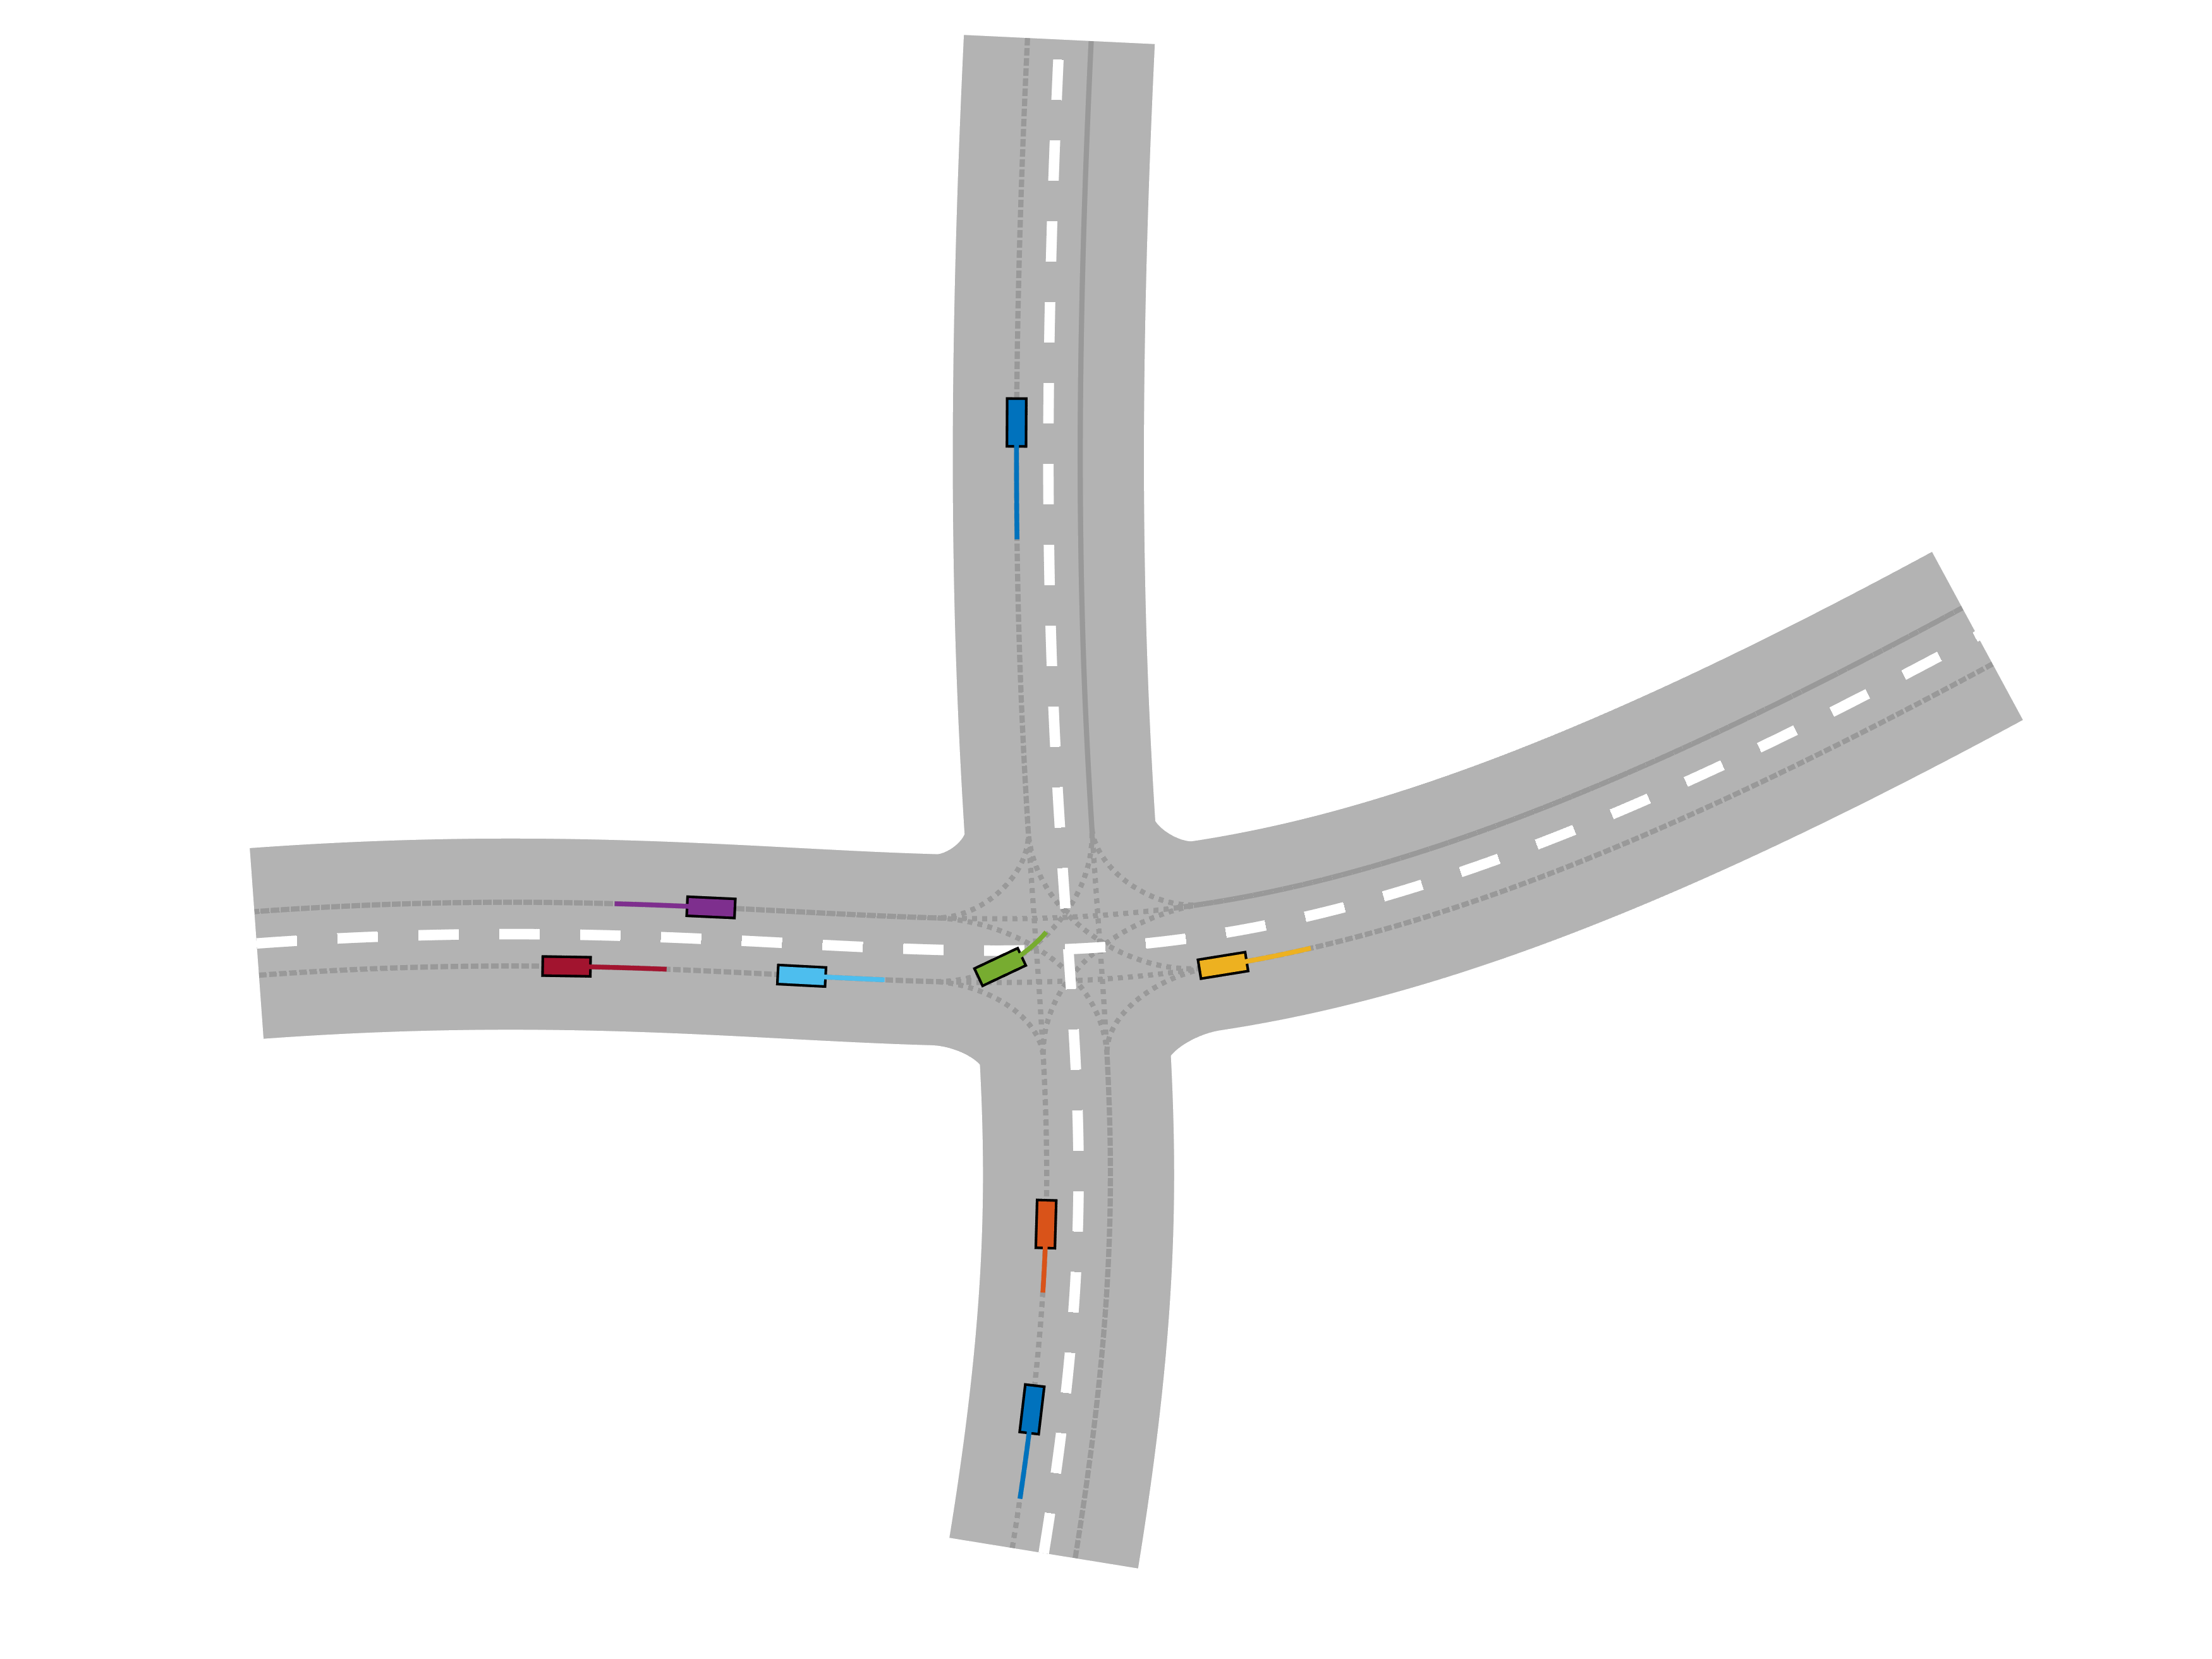
\includegraphics[scale=0.36]{Simulations/frame_crossroad_7.png}}
    \caption{Simulated scenario. The full animation is available as supplementary material.}
    \label{fig:frame_simulation}
\end{figure*}
%%%%%%%%%%%%%%%%%%%%%%%%%
In the latter, $p_i$ denotes the progress (in meters) of vehicle $i$ starting from the entrance point to the intersection, $d_i$ is the desired distance from $\chi(i)$, and $v_i$ denotes the speed. Each vehicle is modelled as a double integrator, discretized with rate $\tau_\text{s}=0.1s$. The matrices defining \eqref{eq:dynamics} are
\begin{align}
    \begin{split}
        A &= \blkdiag(A_i)_{i\in\mc I}, ~\text{where}~ A_i = \begin{cases}
            1 & \text{if} ~i\in\mc L, \\
            \begin{bmatrix}
                1 & \tau_{\text{s}} \\ 0 &1 
            \end{bmatrix} &\text{if} ~i\notin\mc L
        \end{cases} \\
        B_i &= \col(B_{ij})_{j\in\mc I}, ~\text{where}  \\
        B_{ij} &= \begin{cases}
            \begin{bmatrix}
            \tau_\text{s}^2/2 & \tau_\text{s} 
        \end{bmatrix}^\top &\text{if}~ i=\chi(j)\\
        -\begin{bmatrix}
            \tau_\text{s}^2/2 & \tau_\text{s} 
        \end{bmatrix}^\top &\text{if}~ i=j ~\text{and}~ i\notin\mc L \\
        -\tau_\text{s} &\text{if}~ i=j ~\text{and}~ i\in\mc L \\
        0_{1\times 2}  & \text{else}.
        \end{cases}
    \end{split}
\end{align}
In order to satisfy the stabilizability assumption in Assumption \ref{as:objective_system}, each agent applies the pre-stabilizing local controller $K_i$ such that
\begin{equation*}
    % K_ix =-[.1, .1]x_i.
    K_ix =-0.1\cdot \mathds{1}^\top x_i.
\end{equation*}
The constraints include the safety distance and the speed constraints, as well as an input box constraint:
\begin{align*}
    p_{\chi(i)} - p_i \geq d_{\text{min}},\\
    v^{\text{min}} \leq v_i \leq v^{\text{max}},\\
    u^{\text{min}} \leq u_i \leq u^{\text{max}}. 
\end{align*}
The state and input weight matrices are $Q_i=I_n$, $R_i = 1$. We observe in Figure \ref{fig:simulation_result} that all vehicles achieve the desired reference speed and distance, while satisfying the constraints. An animation of the simulated scenario is available as supplementary material, where it is observed that the vehicles safely complete the maneuver. \edit{We illustrate some extracted frames of the animation in Figure \ref{fig:frame_simulation}.} \edit{Figure \ref{fig:simulation_result_convergence} illustrates the efficacy of the splitting method \eqref{DR-affineVI} with the considered setup in \eqref{eq:example_matrix_splitting}. As shown, the number of iterations decreases as the time step increases, and it eventually converges in a single iteration: In consideration of Lemma \ref{lem: inactive cons}, we speculate that the Douglas-Rachford algorithm behaves similarly to a Newton algorithm when constraints are inactive, which ensures convergence in a single iteration for solving linear unconstrained systems. Note that the algorithm is considered to have converged when \( r_k \leq 10^{-4} \), where \( r_k \) is the natural residual at iteration \( k \) of the iterative method \eqref{DR-affineVI} \cite[\S 6.2.1]{facchinei2003finite}.}

\begin{comment}
\begin{figure}
    \centering
    \begin{minipage}{0.49\columnwidth}
        \centering
        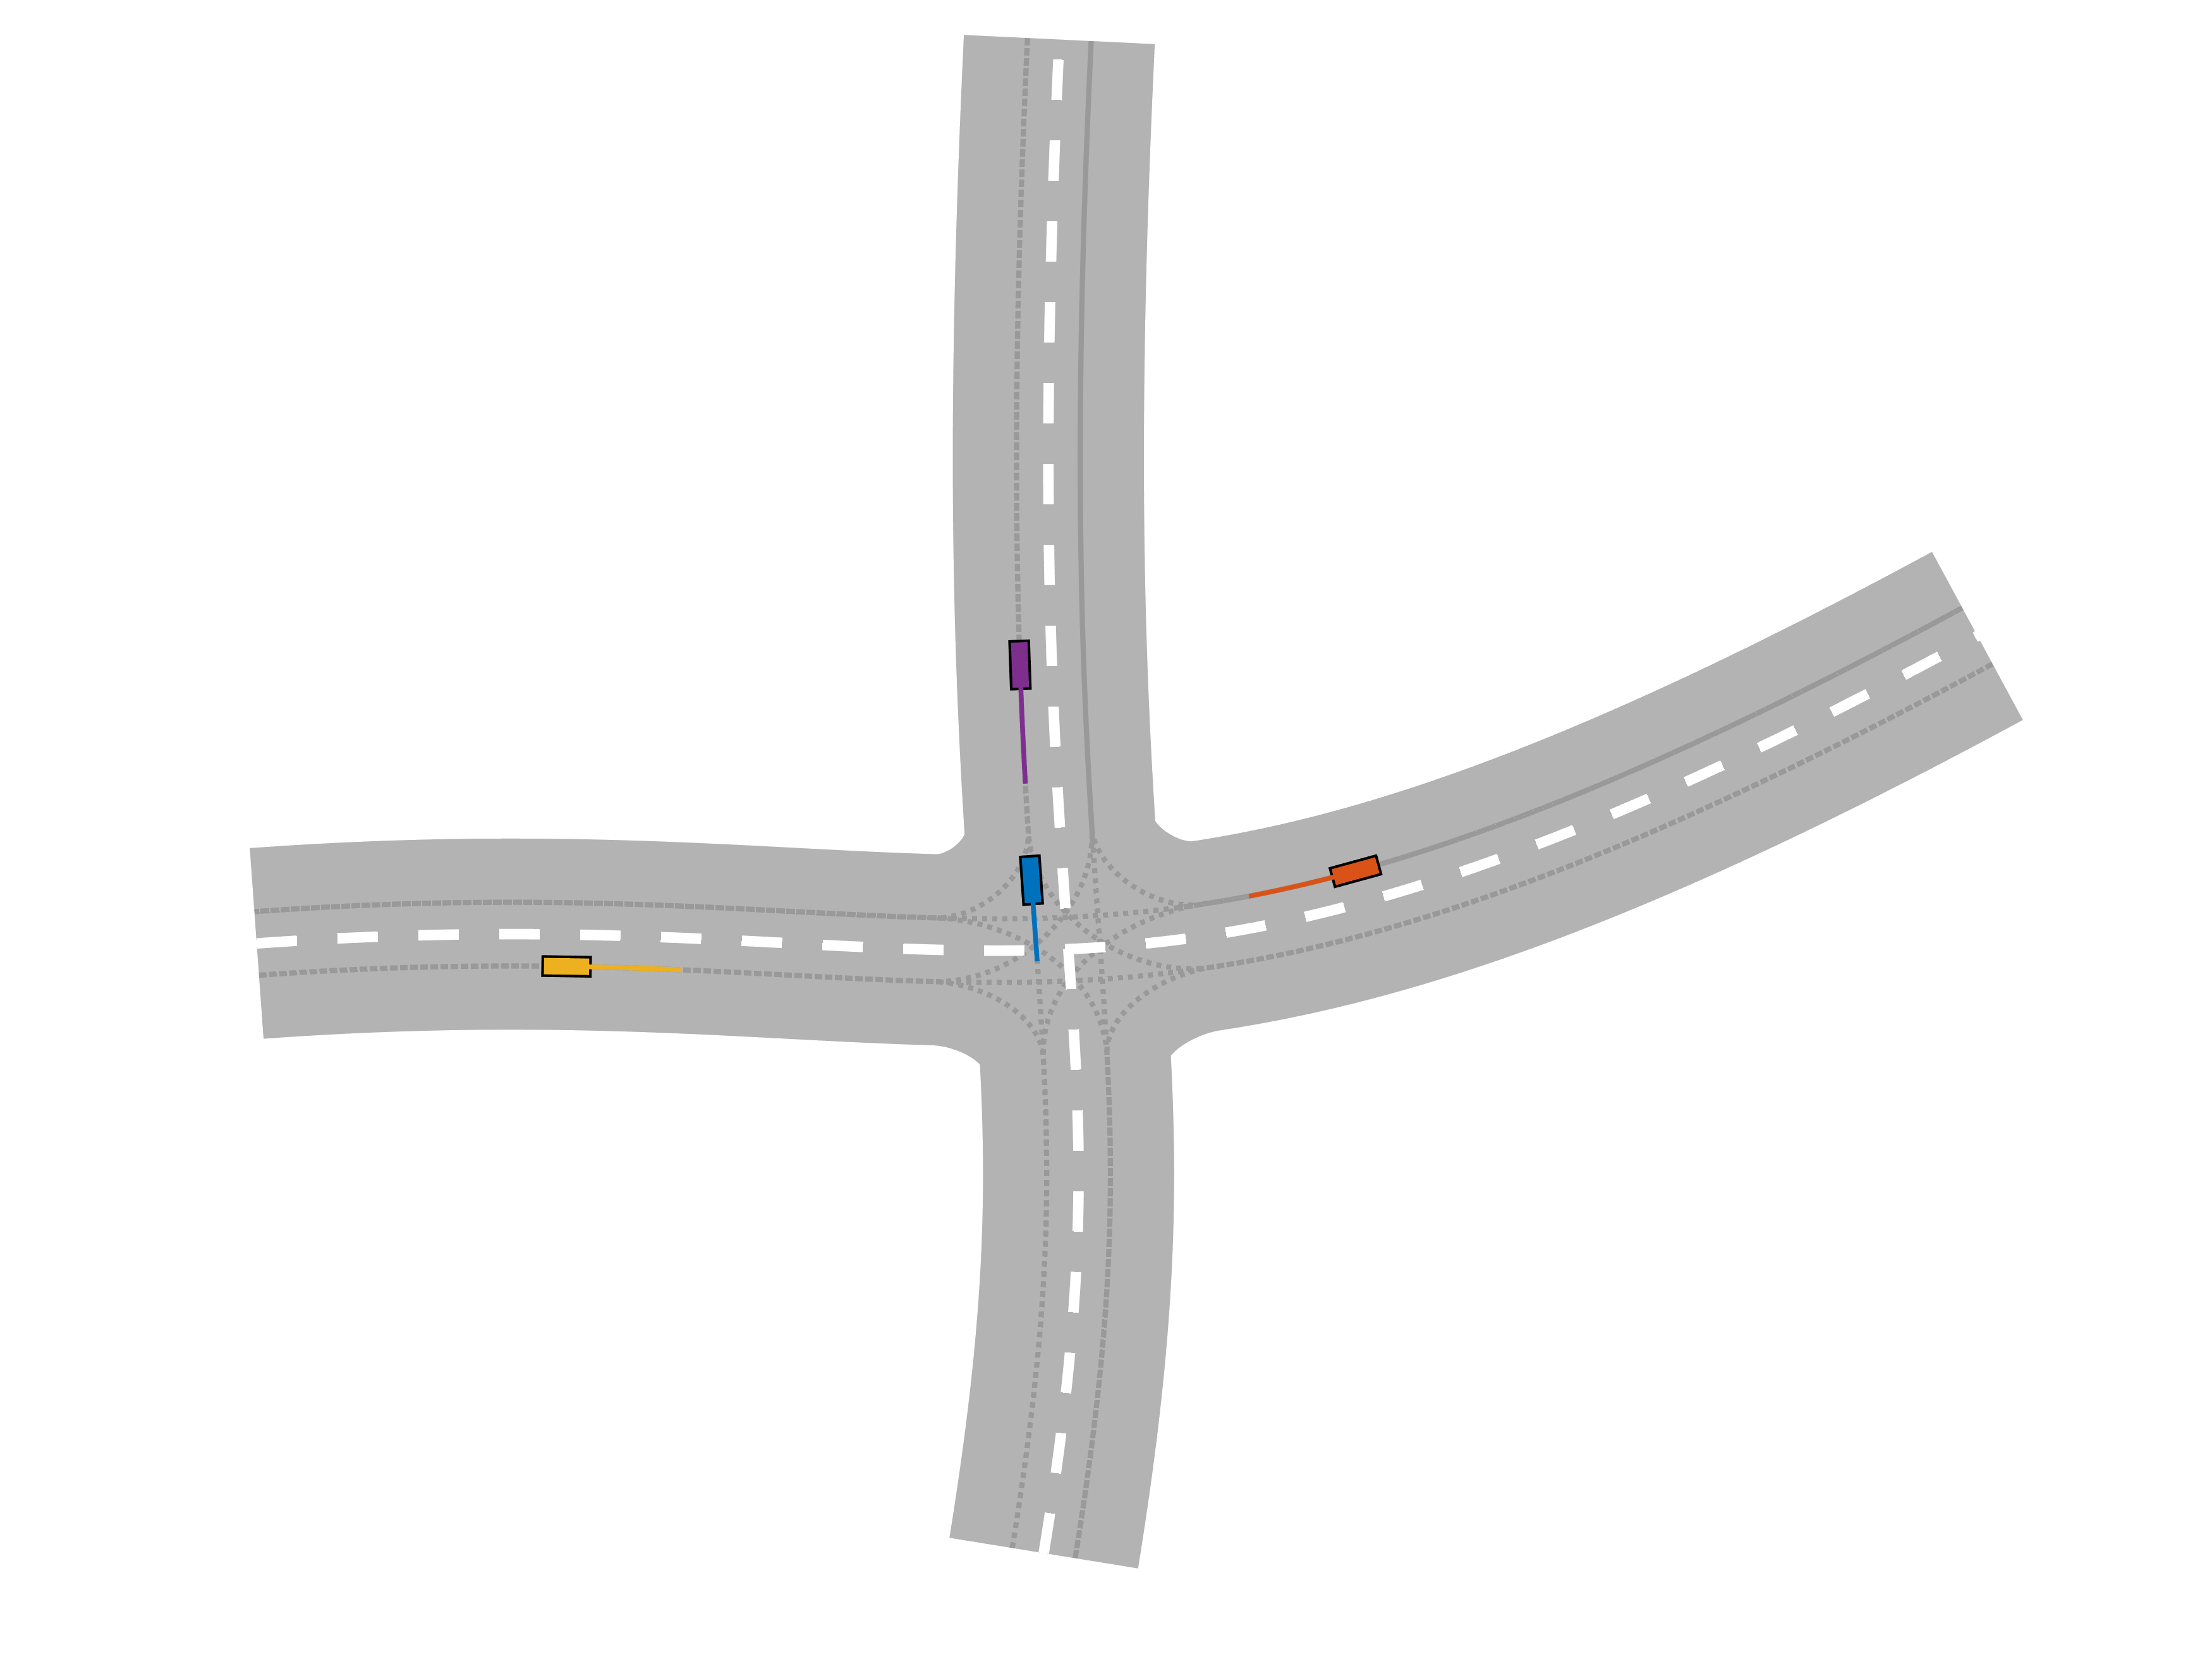
\includegraphics[width=\linewidth]{Simulations/frame_crossroad_3.png}
        \subcaption{Agents 1--4 approach the intersection}
    \end{minipage}
    \begin{minipage}{0.49\columnwidth}
        \centering
        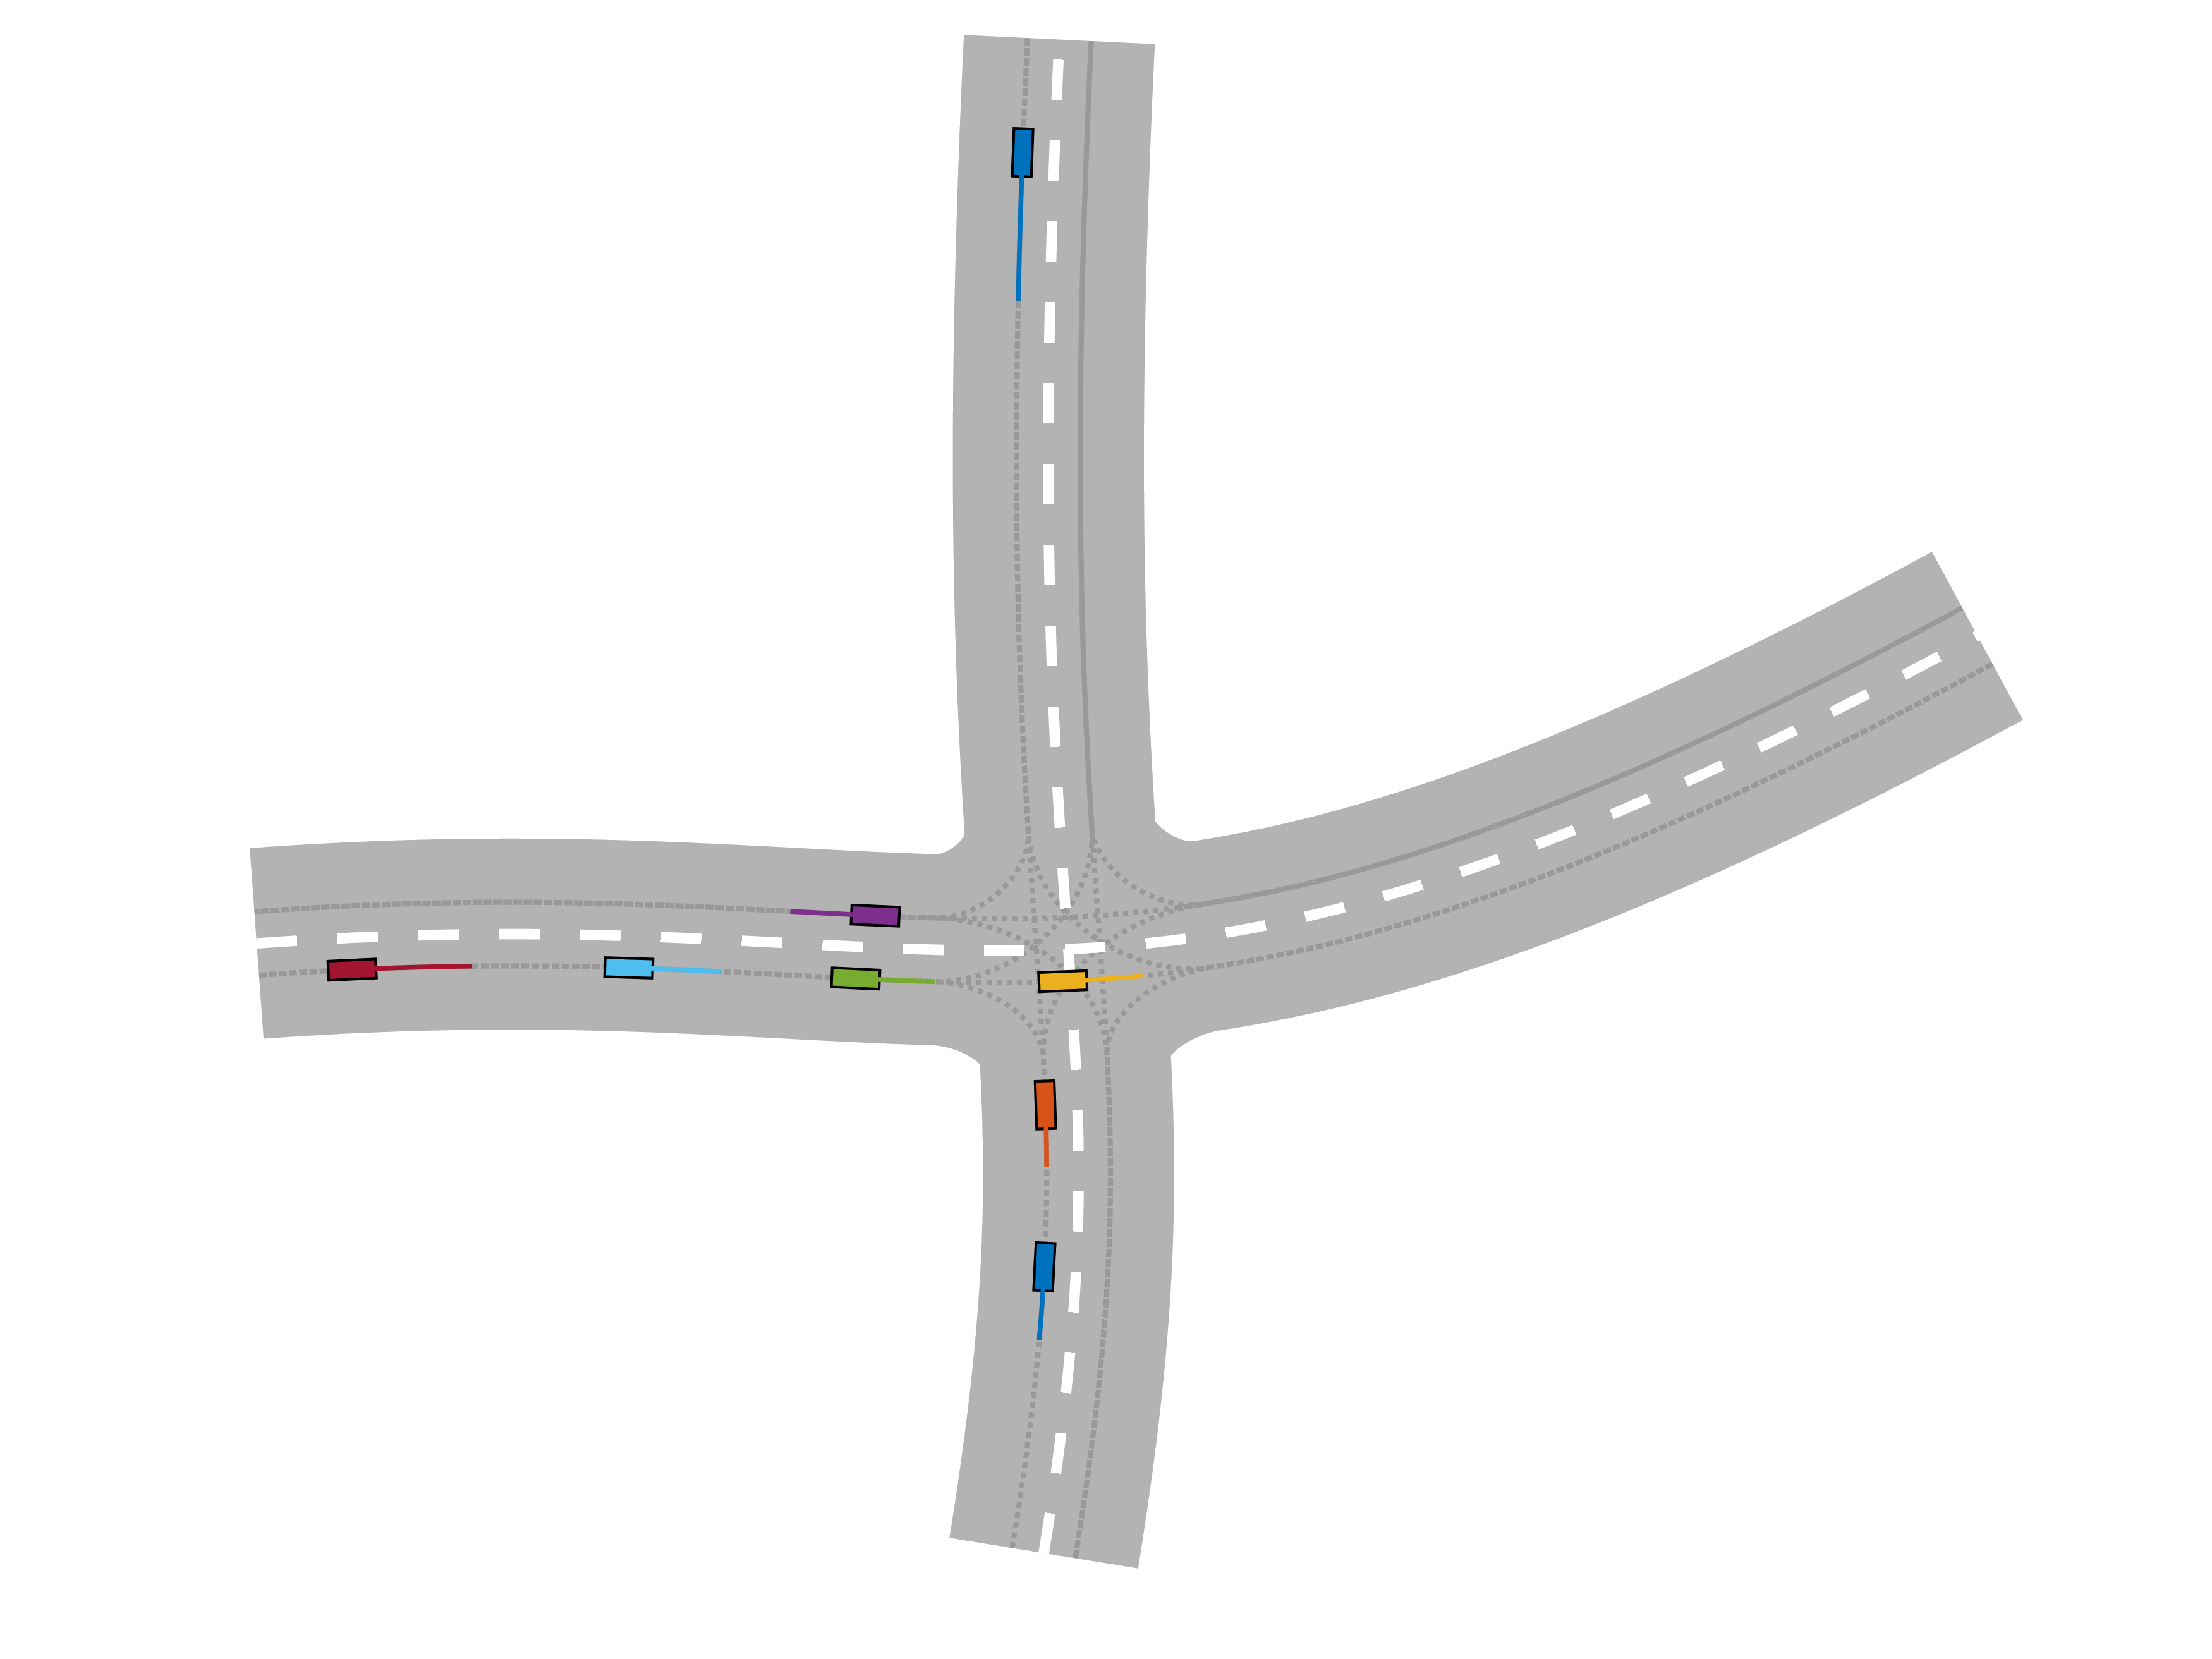
\includegraphics[width=\linewidth]{Simulations/frame_crossroad_6.png}
        \subcaption{Agent 1 (Blue) crosses the intersection first. Agents 2 (orange), and 4 (violet) cross next, contemporarily.}
    \end{minipage}
    
    \vspace{0.5cm}
    
    \begin{minipage}{0.49\columnwidth}
        \centering
        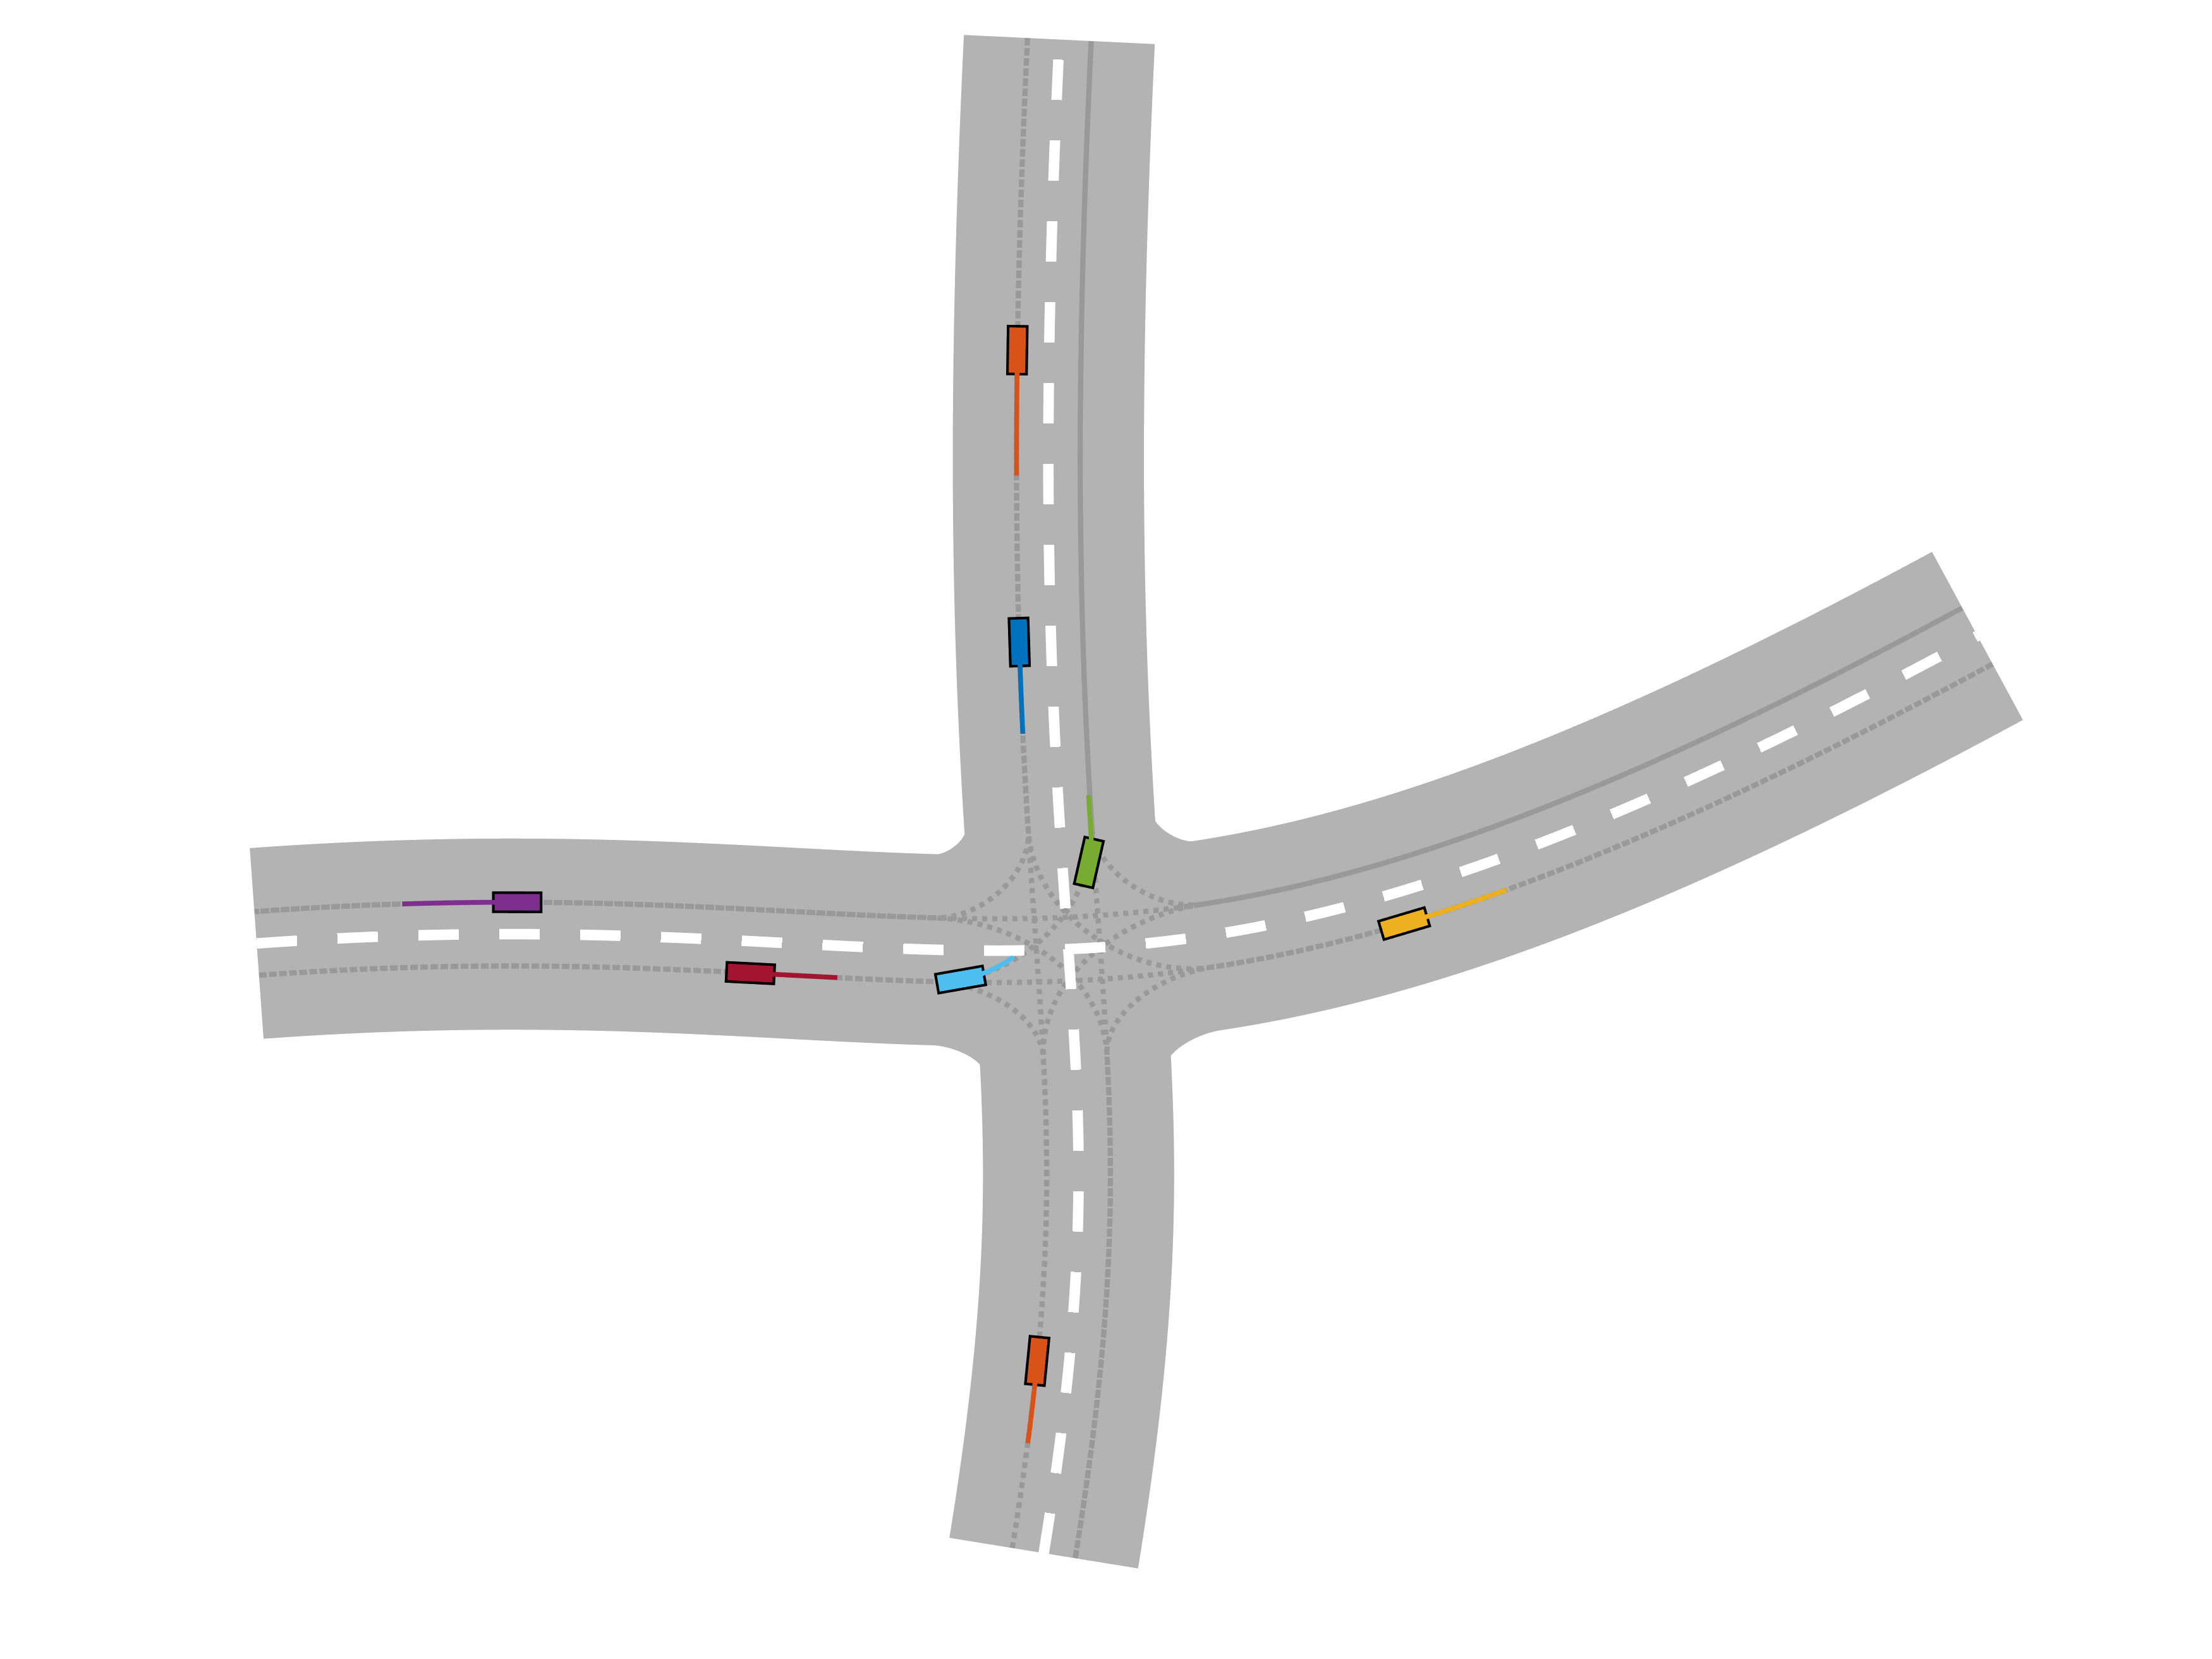
\includegraphics[width=\linewidth]{Simulations/frame_crossroad_8.png}
        \subcaption{Agent 3 (yellow) crosses the intersection, followed by Agent 5 (green).}
    \end{minipage}

    \caption{Simulated scenario. The full animation is available as supplementary material.}
    \label{fig:frame_simulation}
\end{figure}
\end{comment}

\begin{figure}
    \centering
    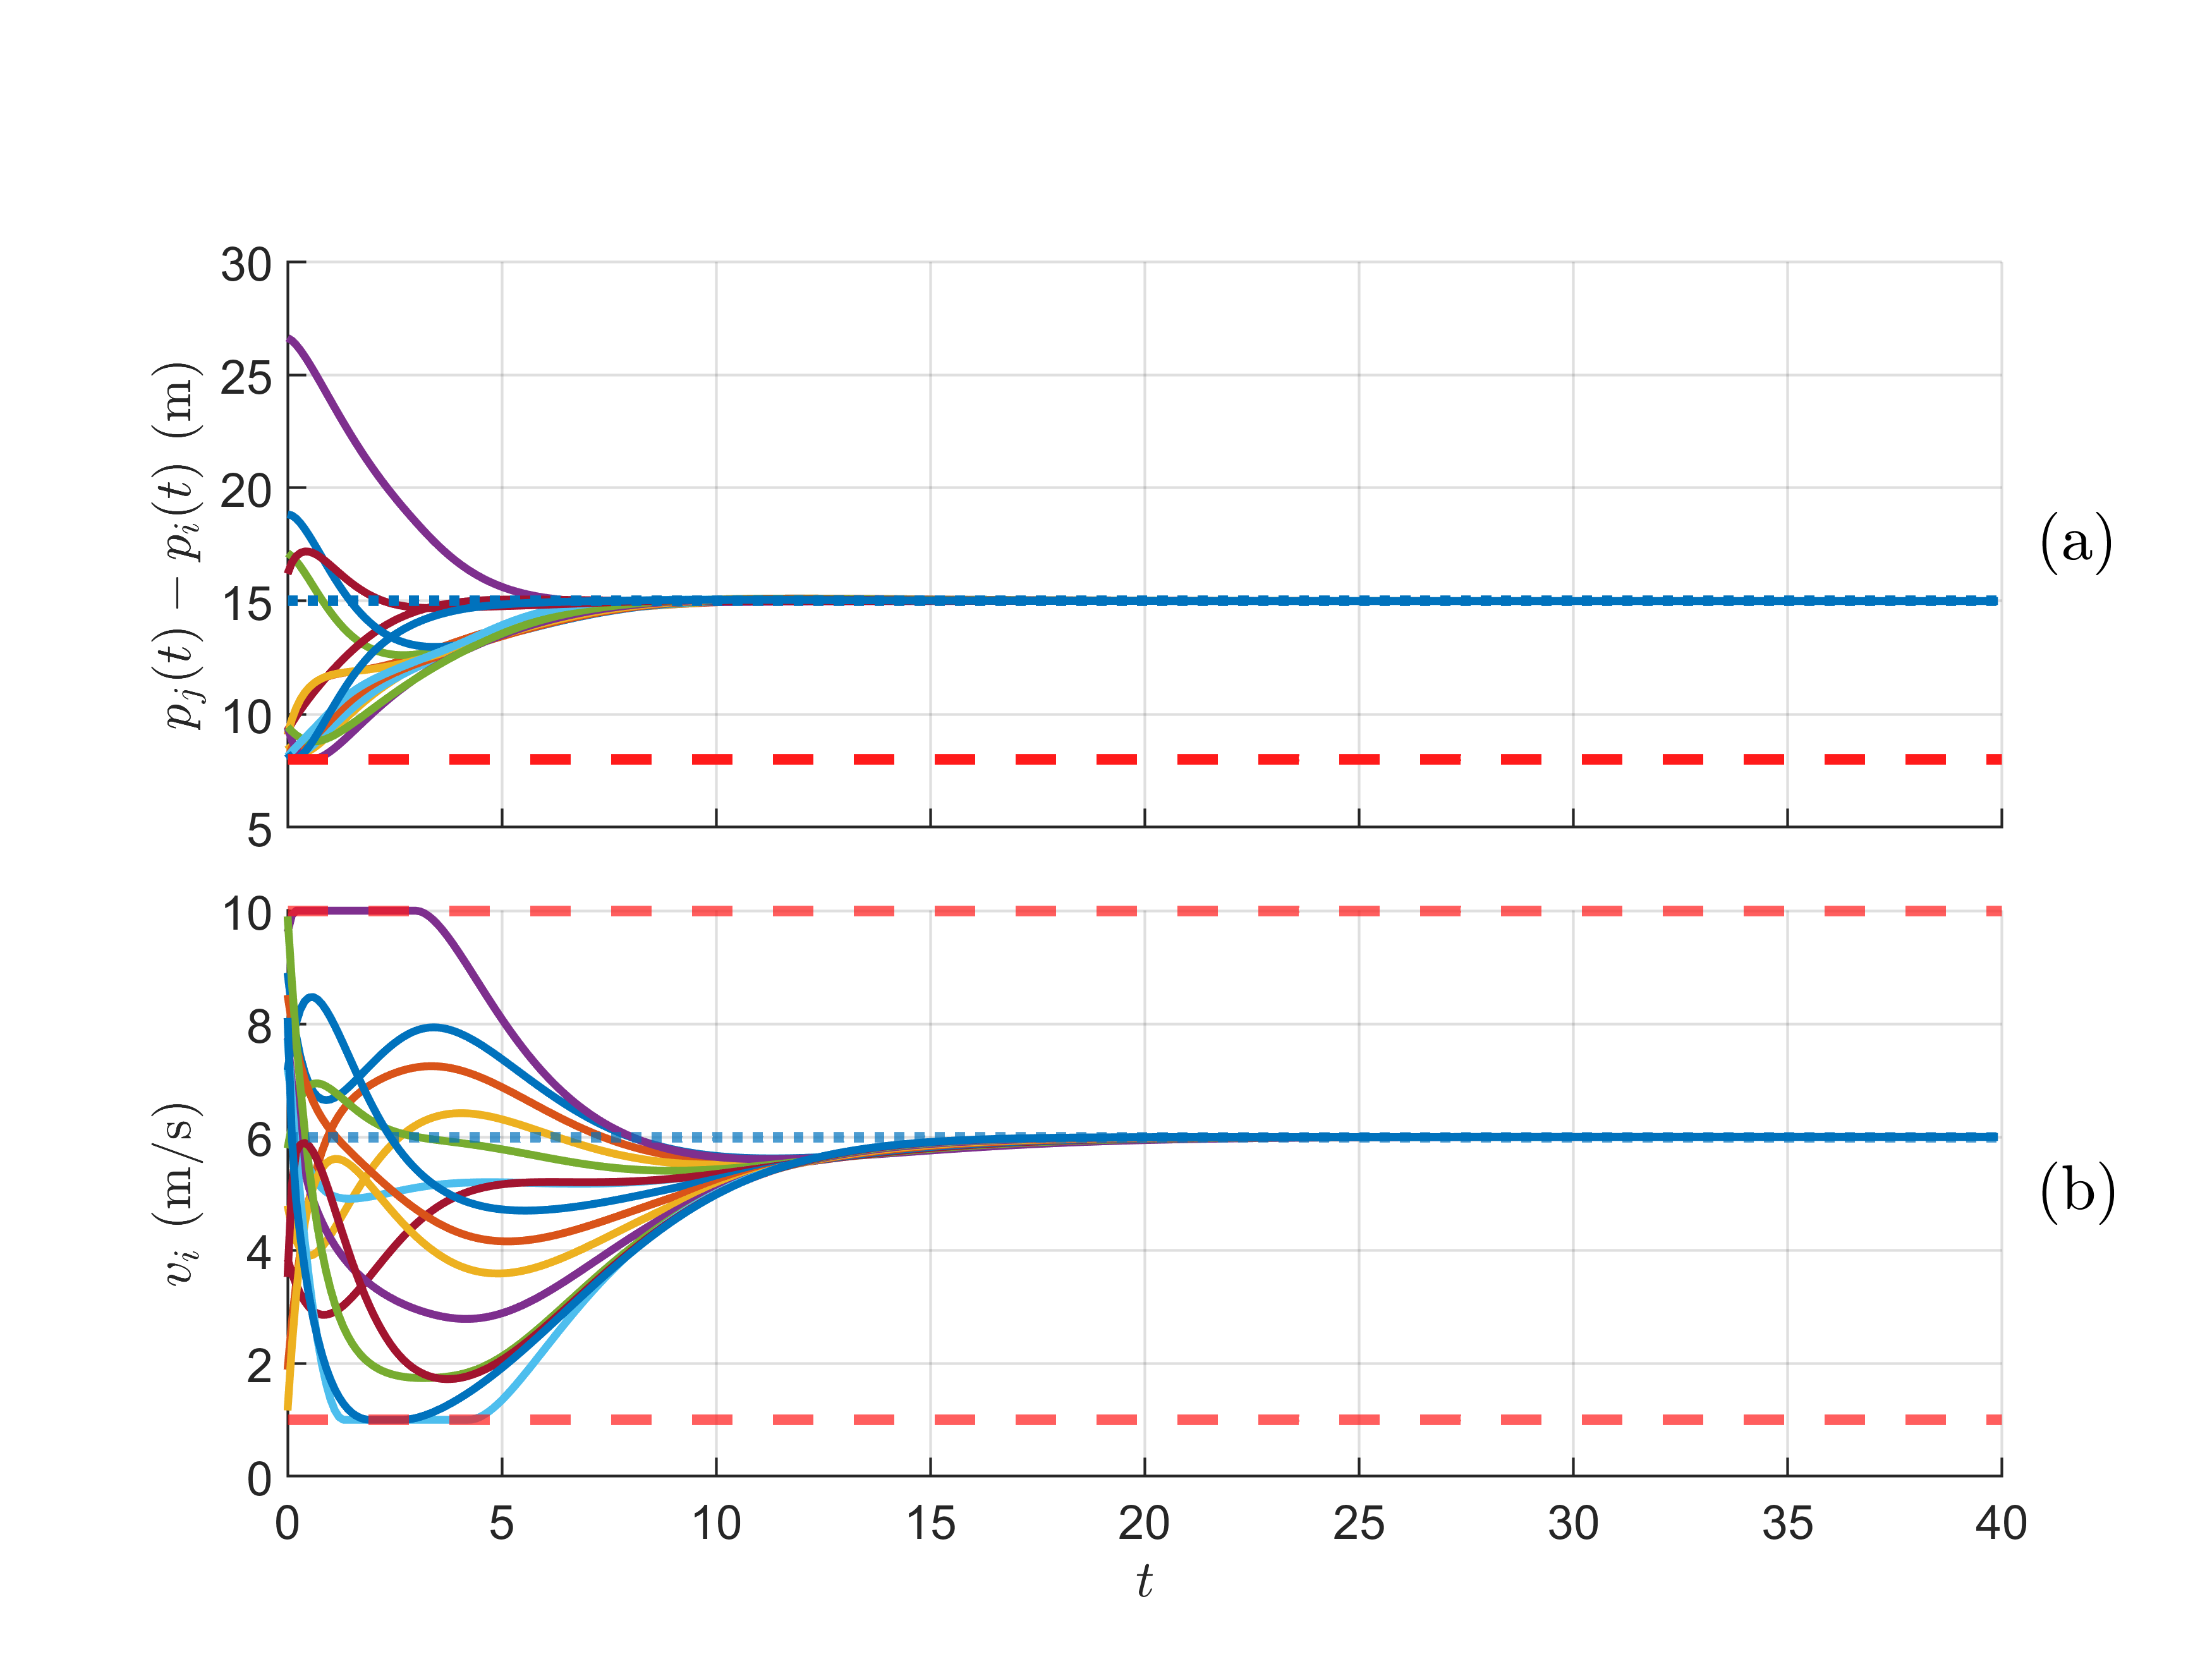
\includegraphics[width=\linewidth]{Simulations/pos_velocity_dist_to_Xf.png}
    \caption{(a): Distance between $\chi(i)$ and $i$. (b): Velocity of each agent. The dotted lines denote the reference values, and the red dashed lines denote the constraints. }
    \label{fig:simulation_result}
\end{figure}

\begin{figure}
    \centering
    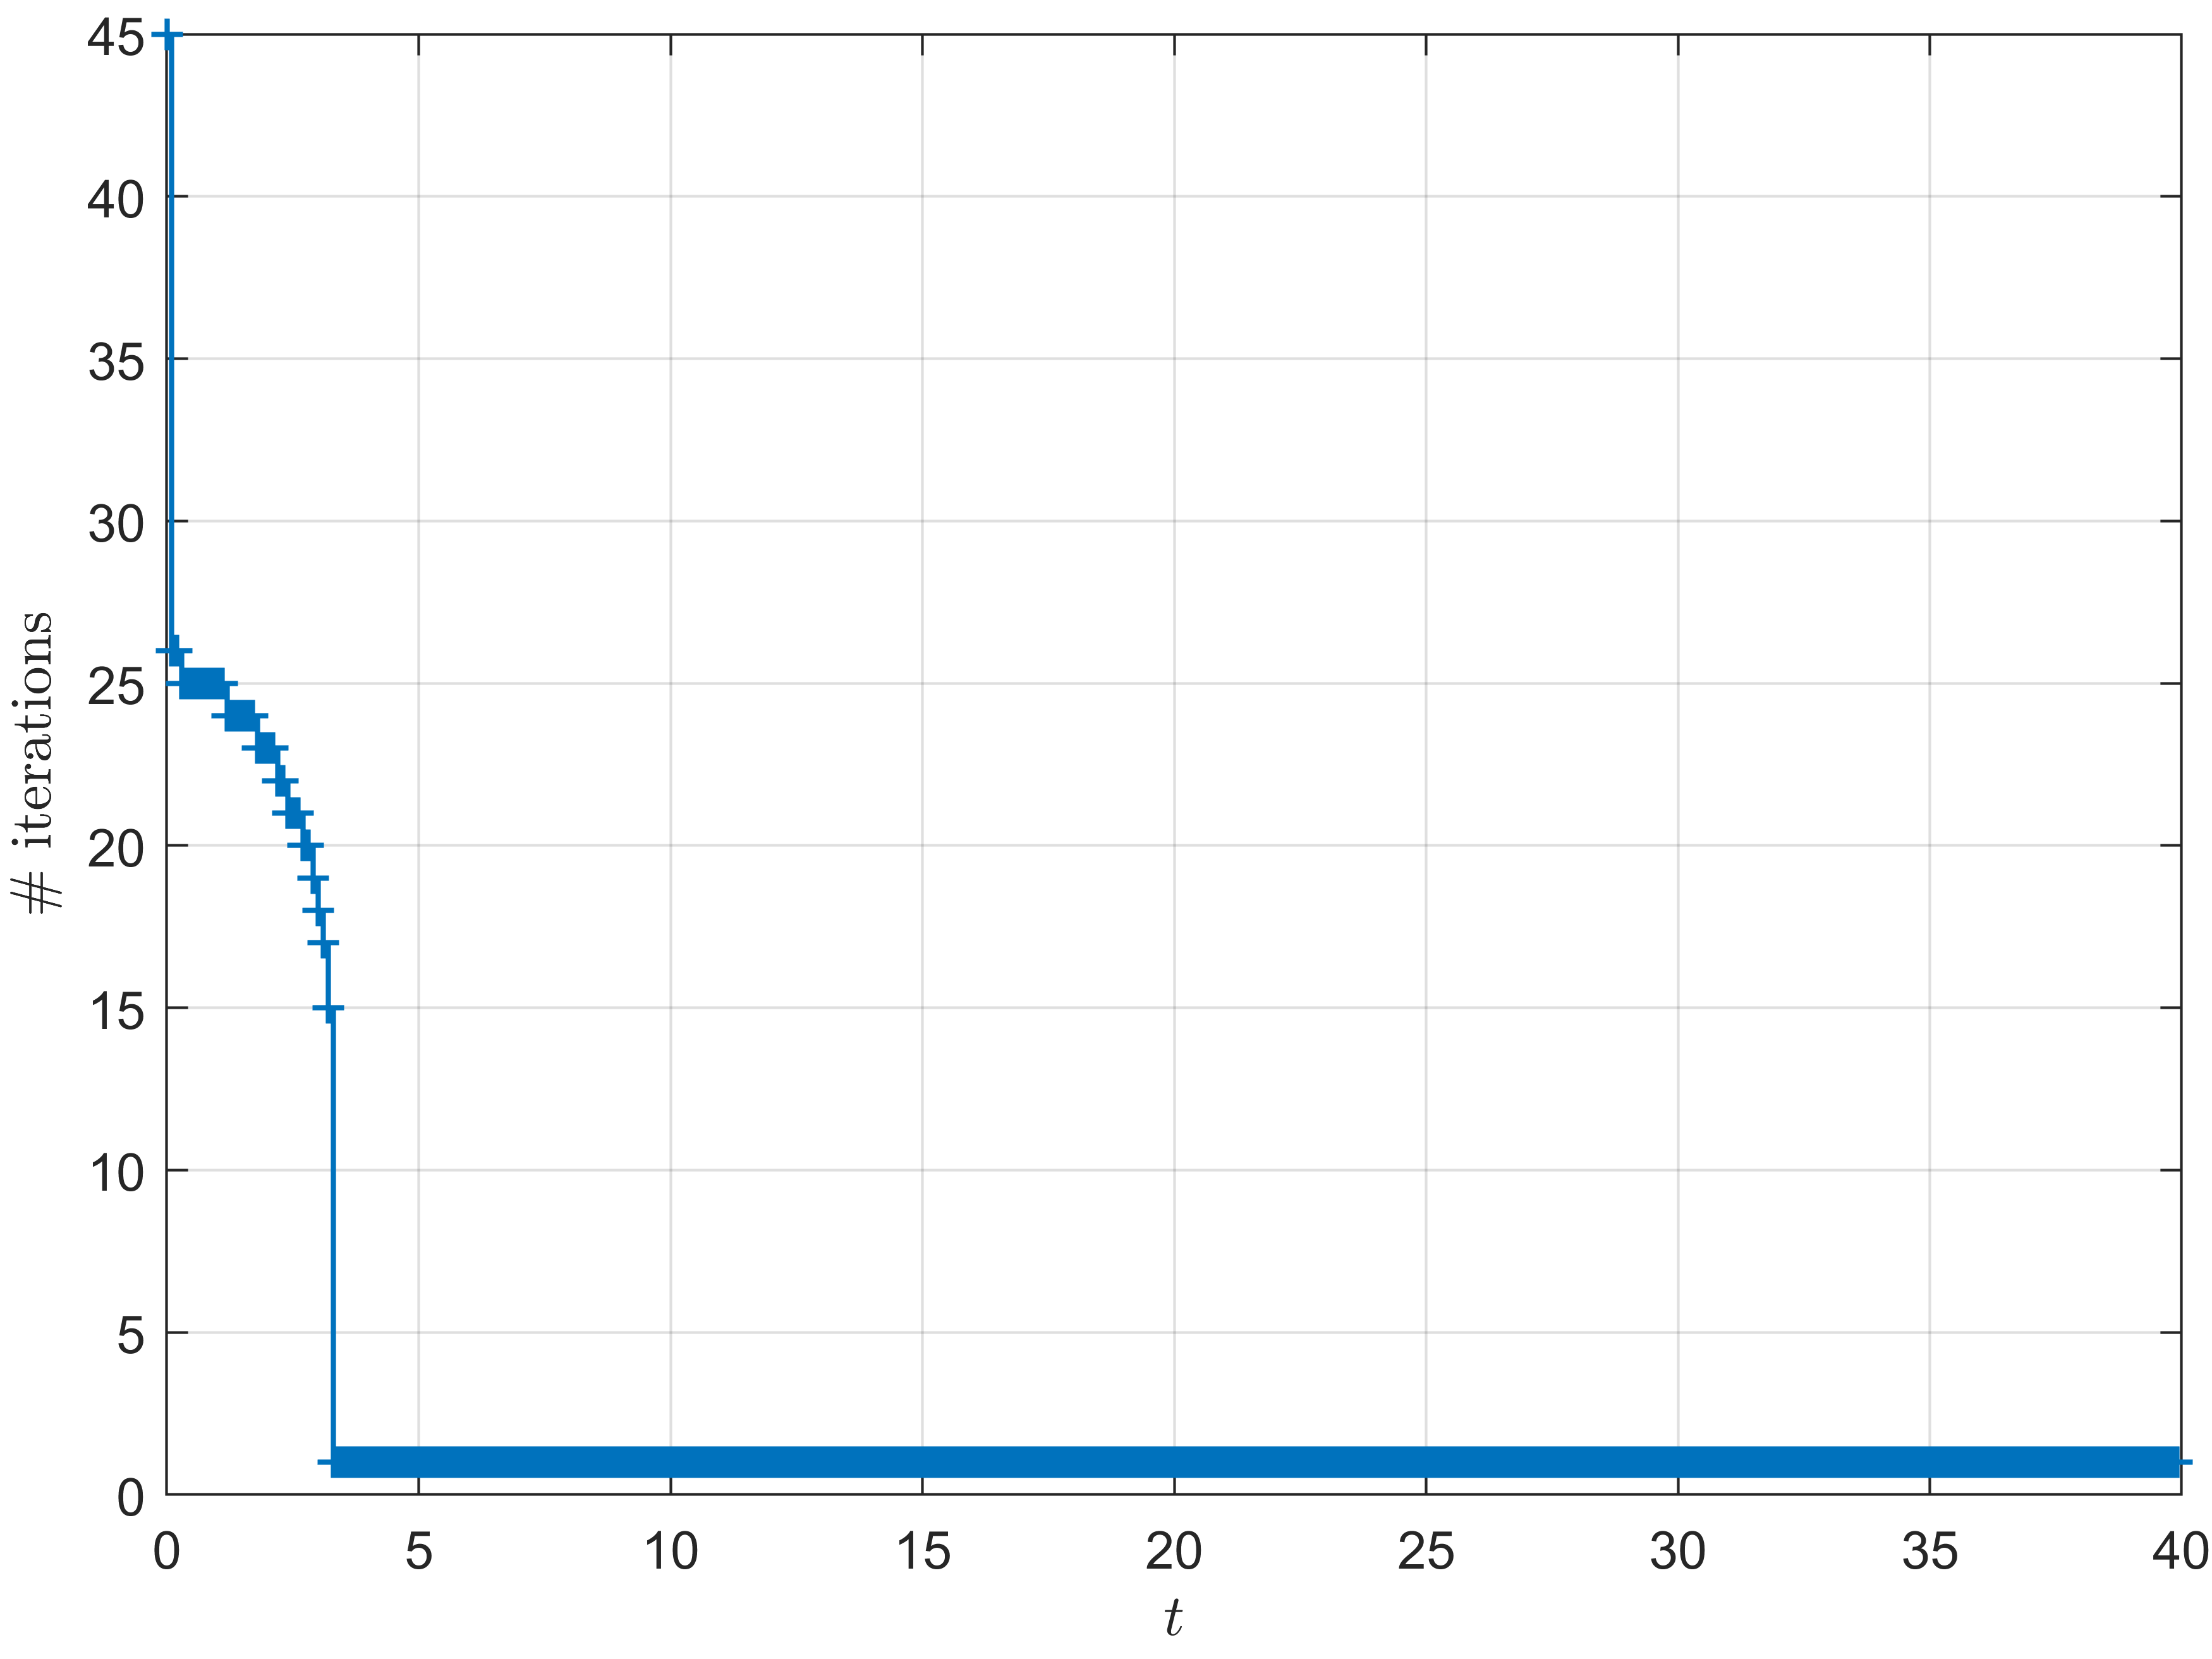
\includegraphics[width=.75\linewidth]{Simulations/num_iter_to_convergence.png}
    \caption{{Number of iterations to achieve convergence of the VI solution algorithm.}} %The algorithm is considered converged when $r_k\leq 10^{-4}$, where $r_k$ is the natural residual at iteration $k$ \cite[\S 6.2.1]{facchinei2003finite}.} }
    \label{fig:simulation_result_convergence}
\end{figure}

%%%%%%%%%%%%%%%%%%%%%%%%%%%%%%%%%%%%%%%%%%%%%%%%%%%%%%%%%%%%%%%%%%%%%%%%%%%%%%%%
\section{Conclusion}\label{sec: conclusion}
For linear-quadratic dynamic games, an open-loop Nash equilibrium is the solution to an affine variational inequality, if the terminal state belongs to a forward-invariant, constraint-admissible set for the infinite-horizon unconstrained Nash equilibrium. This enables receding-horizon game-theoretic control architectures, which require a fast solution of the variational inequality. The Douglas-Rachford splitting-like method is particularly suited for this application, as it shows a remarkable linear convergence speed. Additionally, considering that constraints are typically inactive near the equilibrium attractor of the dynamic game, \edit{the computational effort required to solve the associated VI is further reduced. Therefore, thanks to the proposed algorithm, which requires very few iterations to converge, solving variational inequalities in real-time is now a reality.} Future work will investigate other applications of real-time control for multi-agent robotic systems based on receding-horizon variational inequalities.


% We illustrate a potential application by testing the method on a receding-horizon controller for navigating a fleet of vehicles across an intersection.

% Finally, the effectiveness of the proposed algorithm is demonstrated through a receding-horizon control method applied to autonomous vehicle navigation at a crossroad, a key application in autonomous driving.
%%%%%%%%%%%%%%%%%%%%%%%%%%%%%%%%%%%%%%%%%%%%%%%%%%%%%%%%%%%%%%%%%
\section{Appendix}\label{appendix}

\subsection{State-of-the-art algorithms for solving (strongly)~monotone variational inequalities} \label{algorithm review}
We review some recent and closely related existing methods for solving \eqref{VI-main}.\\
%%%%%%%%%%%%%%%%%%%%%%%%%%%%%%%
\textbf{Projected Gradient Descent (PGD) \cite{nemirovskij1983problem}:}  
\begin{align*}
    u^{k+1} &= \pi_{\mathcal{C}}(u^k - \lambda F(u^k)),
\end{align*}
where \(\lambda\) is the stepsize. This method guarantees convergence for strongly monotone operators (with constant \(\mu\)) and Lipschitz operators (with constant \(L\)) when \(\lambda \in (0, 2\mu/L^2)\).\\
\textbf{Extragradient Descent ({EXGD}) \cite{malitsky2014extragradient}:}
\begin{align*}
    y^k &= \pi_{\mathcal{C}}(u^k - \lambda F(u^k)), \\
    u^{k+1} &= \pi_{\mathcal{C}}(u^k - \lambda F(y^k)),
\end{align*}
with \(\lambda\) as the stepsize. Unlike PGD, this method ensures convergence for Lipschitz operators (with constant \(L\)) when \(\lambda \in (0, 1/L)\). \\
\textbf{Nesterov's accelerated gradient descent ({NAGD}) \cite{nesterov2006solving}:}
\begin{align*}
    u^k &= \arg\max_{u \in \mathcal{C}} \, \sum_{i=0}^k \lambda_i \left[\langle F(y^i), y^i - u \rangle - \frac{\mu}{2} \|u - y^i\|^2\right], \\
    y^{k+1} &= \arg\max_{u \in \mathcal{C}} \, \langle F(u^k), u^k - u \rangle - \frac{\beta}{2} \|u - u^k\|^2,
\end{align*}
where \(\lambda_{k+1} = \frac{\mu}{L} \sum_{i=0}^k \lambda_i\) is the stepsize at iteration \(k+1\). This method guarantees convergence for strongly monotone operators (with constant \(\mu\)) and \(\beta = L\), where \(L\) is the Lipschitz constant of the operator \(F\).\\
\textbf{Projected Reflected Gradient Descent ({PRGD}) \cite{malitsky2015projected}:}  
\begin{align*}
    u^{k+1} &= \pi_{\mathcal{C}}(u^k - \lambda F(2u^k - u^{k-1})),
\end{align*}
where \(\lambda\) is the stepsize. This method guarantees convergence for a Lipschitz operator (with constant \(L\)) when \(\lambda \in (0, (\sqrt{2}-1)/L)\). Unlike the extragradient method, it requires only one projection per iteration.\\
\textbf{Golden Ratio Algorithm (GRAAL) \cite{malitsky2020golden}:}  
\begin{align*}
    y^k &= (1-\beta)u^k + \beta y^{k-1}, \\
    u^{k+1} &= \pi_{\mathcal{C}}(y^k - \lambda F(u^k)),
\end{align*}
with \(\lambda\) as the stepsize and \(\beta \in \left(0, (\sqrt{5}-1)/2\right]\). This method ensures convergence for Lipschitz operators (with constant \(L\)) when \(\lambda \in (0, 1/(2\beta L))\) and requires one projection per iteration. Additionally, the stepsize can be chosen adaptively, leading to the Adaptive Golden Ratio Algorithm (aGRAAL) \cite{malitsky2020golden}: 
\begin{align*}
    \lambda_k &= \min\left\{(\beta + \beta^2)\lambda_{k-1}, \frac{\|u^k - u^{k-1}\|^2}{4\beta^2\lambda_{k-2}\|F(u^k) - F(u^{k-1})\|^2}\right\}.
\end{align*}
\textbf{{Operator splitting methods (DR)} \cite{facchinei2003finite}:}\\
In these types of methods, the operator \( F \) can be split into a summation of different operators. Then, solving \(\mathrm{VI}(\mathcal{C}, F)\) is equivalent to solving \(0 \in F_1 + F_2\), where \(F + \mathcal{N} = F_1 + F_2\), and the iterative update of each sub-operator leads to convergence towards the solution. A famous class of these algorithms is the Douglas-Rachford splitting method, which can be written as:
\begin{align*}
   y^{k+1} &= (I + \lambda F_2)^{-1}\left(u^k - \lambda F_1(u^k)\right), \\
   u^{k+1} &= u^k + \gamma(y^{k+1} - u^k),
\end{align*}
where $\gamma \in (0,2)$ is a relaxation parameter. The convergence of this method is guaranteed for different cases of $F_1$ and $F_2$; we refer interested readers to~\cite{giselsson2017tight,moursi1805douglas} for further details.

{For more algorithms and applications in monotone variational inequalities, we refer interested readers to \cite{mignoni2025monviso} and the references therein.}
%%%%%%%%%%%%%%%

\bibliographystyle{IEEEtran}
\bibliography{IEEEabrv, reference}

\end{document}
